\documentclass{article}
\usepackage{graphicx}
\usepackage{authblk}
\usepackage{amsmath}
\usepackage{listings}

\begin{document}


\title{THEORETICAL NEUROSCIENCE II \\ EXERCISE 05}
\date{21 Mai. 2013}
\author[1]{Yunus Emre Demiray, Taygun C. Uzuneser, \c{S}eyma Bayrak\thanks{seyma.bayrak@st.ovgu.de}}
\affil[1]{\footnotesize  Otto von Guericke University of Magdeburg}
\maketitle

\newpage

\section{Basic Network Description}
Given a population of $N=20-200$ neurons respond to sound frequencies $v$ in the following way:
\begin{equation}
 R_{L,i}=R_{max}\text{exp}(-\dfrac{(v_{pref,L,i}-v)^2}{2\kappa^2v_{pref,L,i}^2})+\eta_i
\end{equation}
where $L$ stands for linearity, with standard deviation $\sigma=\kappa v_{pref,L,i}$, which is proportional to the preferred frequency $v_{pref,L,i}$, the index of neurons $i$ is given such that $i={1,2,...,N}$, the maximum firing response is $R_{max}$,and finally $\eta_i$ is the Gaussian distributed noise for each neuron with a zero mean. The $v_{pref,L,i}$ is chosen randomly between [0,$v_{max}$], where $v_{max}=$1000 Hz. This population is called as the \textit{upstream population}, the key point here is that the standard deviation is not constant, it alters with the preferred frequency $v_{pref,L,i}$ with each neuron.

Another population of $M=20-200$ neurons called \textit{downstream population} has the similar notation in its response formula in the following way:
\begin{equation}
 R_{C,j}=R_{max}\text{exp}(-\dfrac{(v_{pref,C,j}-v)^2}{2\sigma^2})+\eta_j
\end{equation}
where the standard deviation $\sigma$ is now defined to be constant, and the neuron index is given by $j=1,2,...,M$. The preferred frequency is chosen in the same way as in upstream population.

The first task is to define the parameters for both neuron populations, pretend them to be independent of each other and observe their response functions both with and without the noisy parts.

\begin{center}
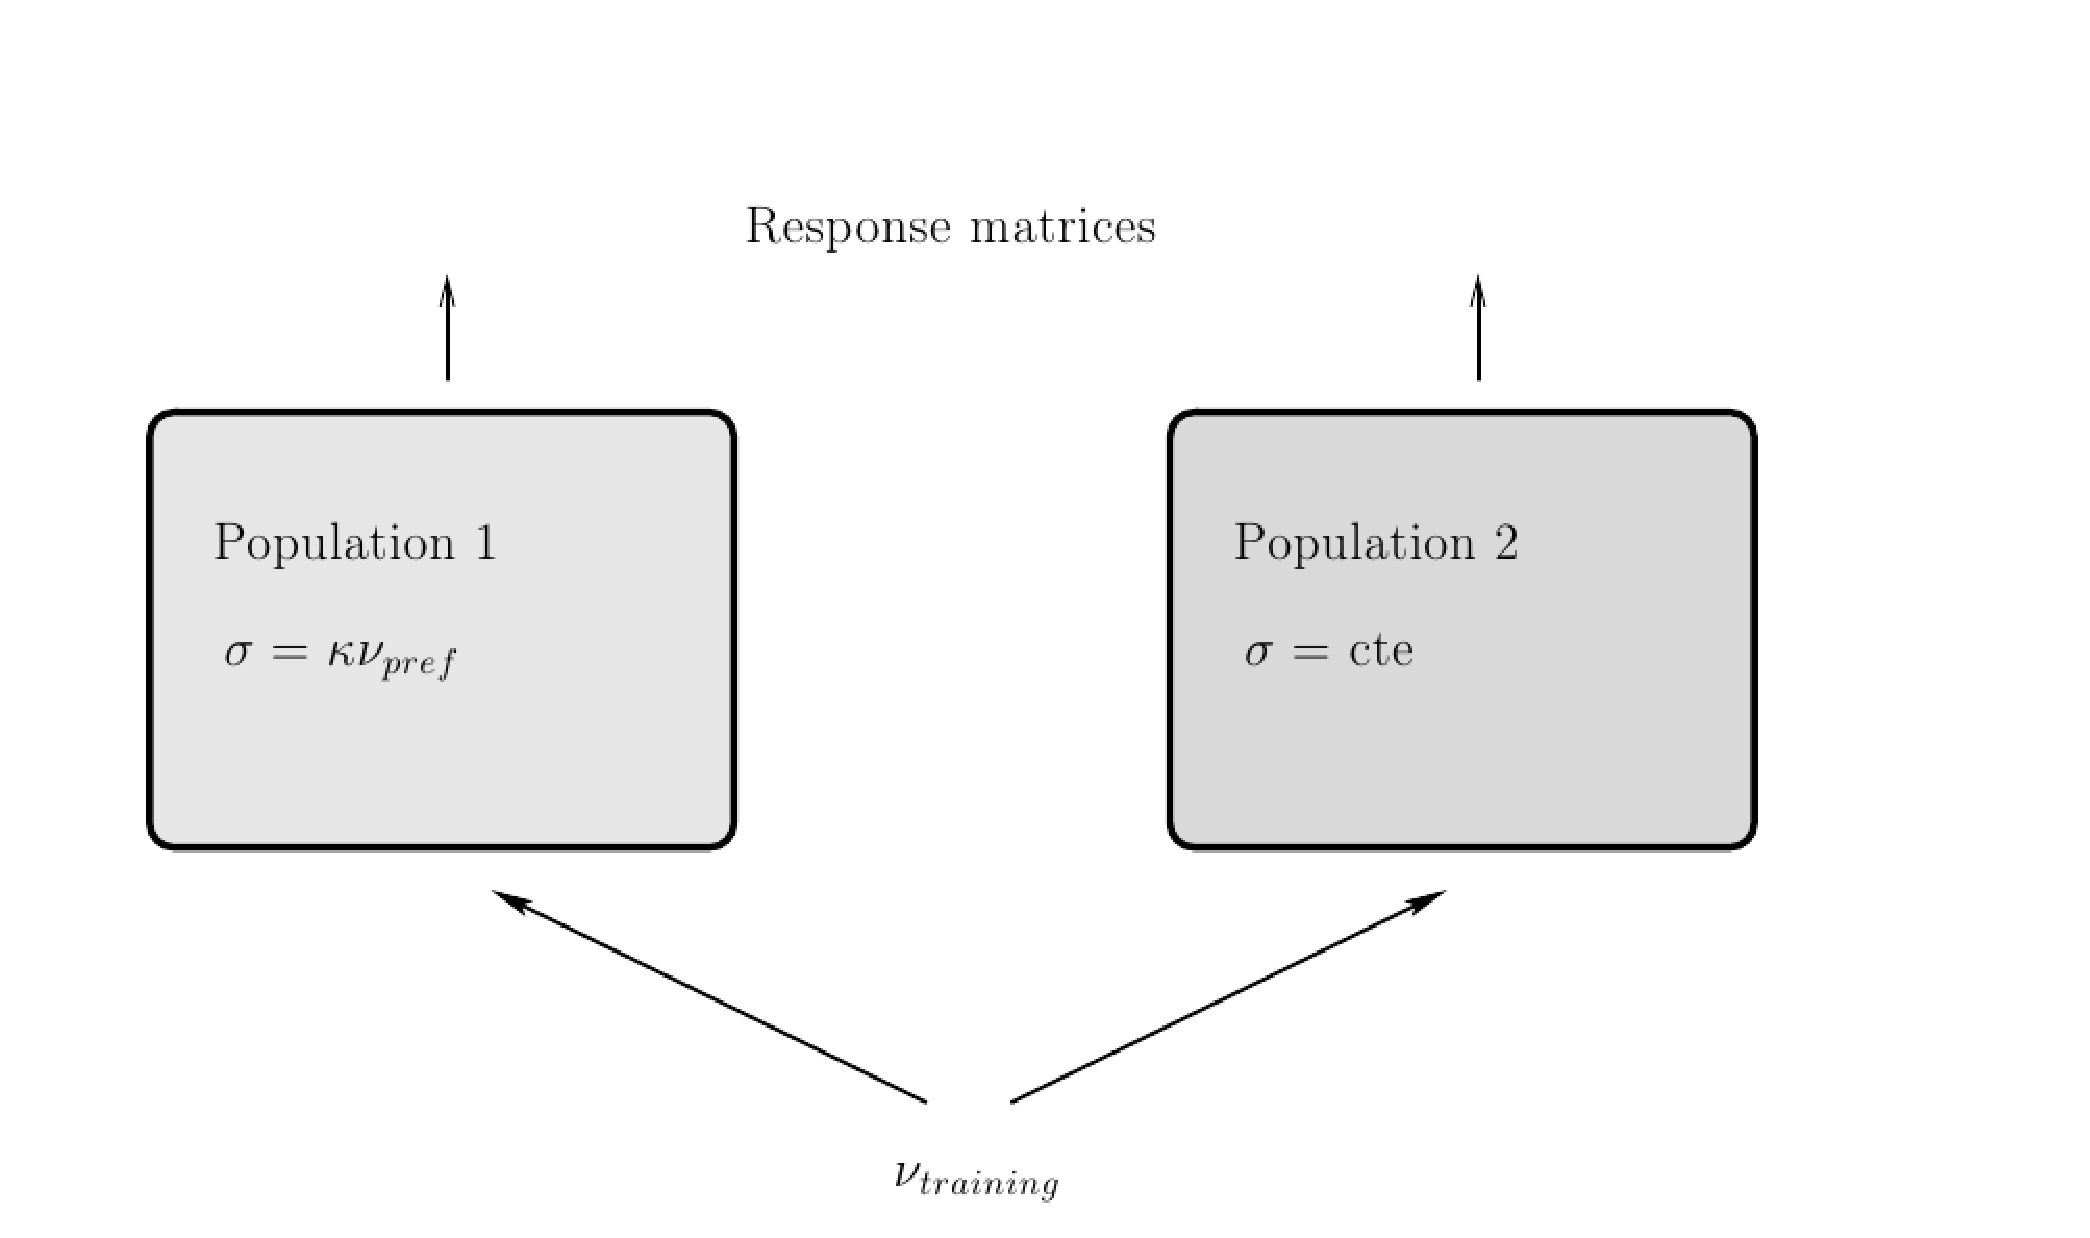
\includegraphics[width=\textwidth]{schema1.eps}
% tau4_M1.eps: 0x0 pixel, 300dpi, 0.00x0.00 cm, bb= -304   -42   918   834
\begin{footnotesize}
 Figure 1, Schematic description of two independent populations, here $v_{training}$ refers to $v$ in actuality
\end{footnotesize}
\end{center}


\begin{itemize}
 \item Parameters: $R_{max}=1$, $\kappa=0.1$, $\sigma=50$, N=40, M=50, two different random preferred frequencies $v_{pref,L,i}$ and $v_{pref,C,j}$ for both populations between 0 and 1000 Hz, the same set of input frequency $v$ for both populations, again randomly and between the interval of 0 and 1000 Hz.
\end{itemize}

\begin{center}
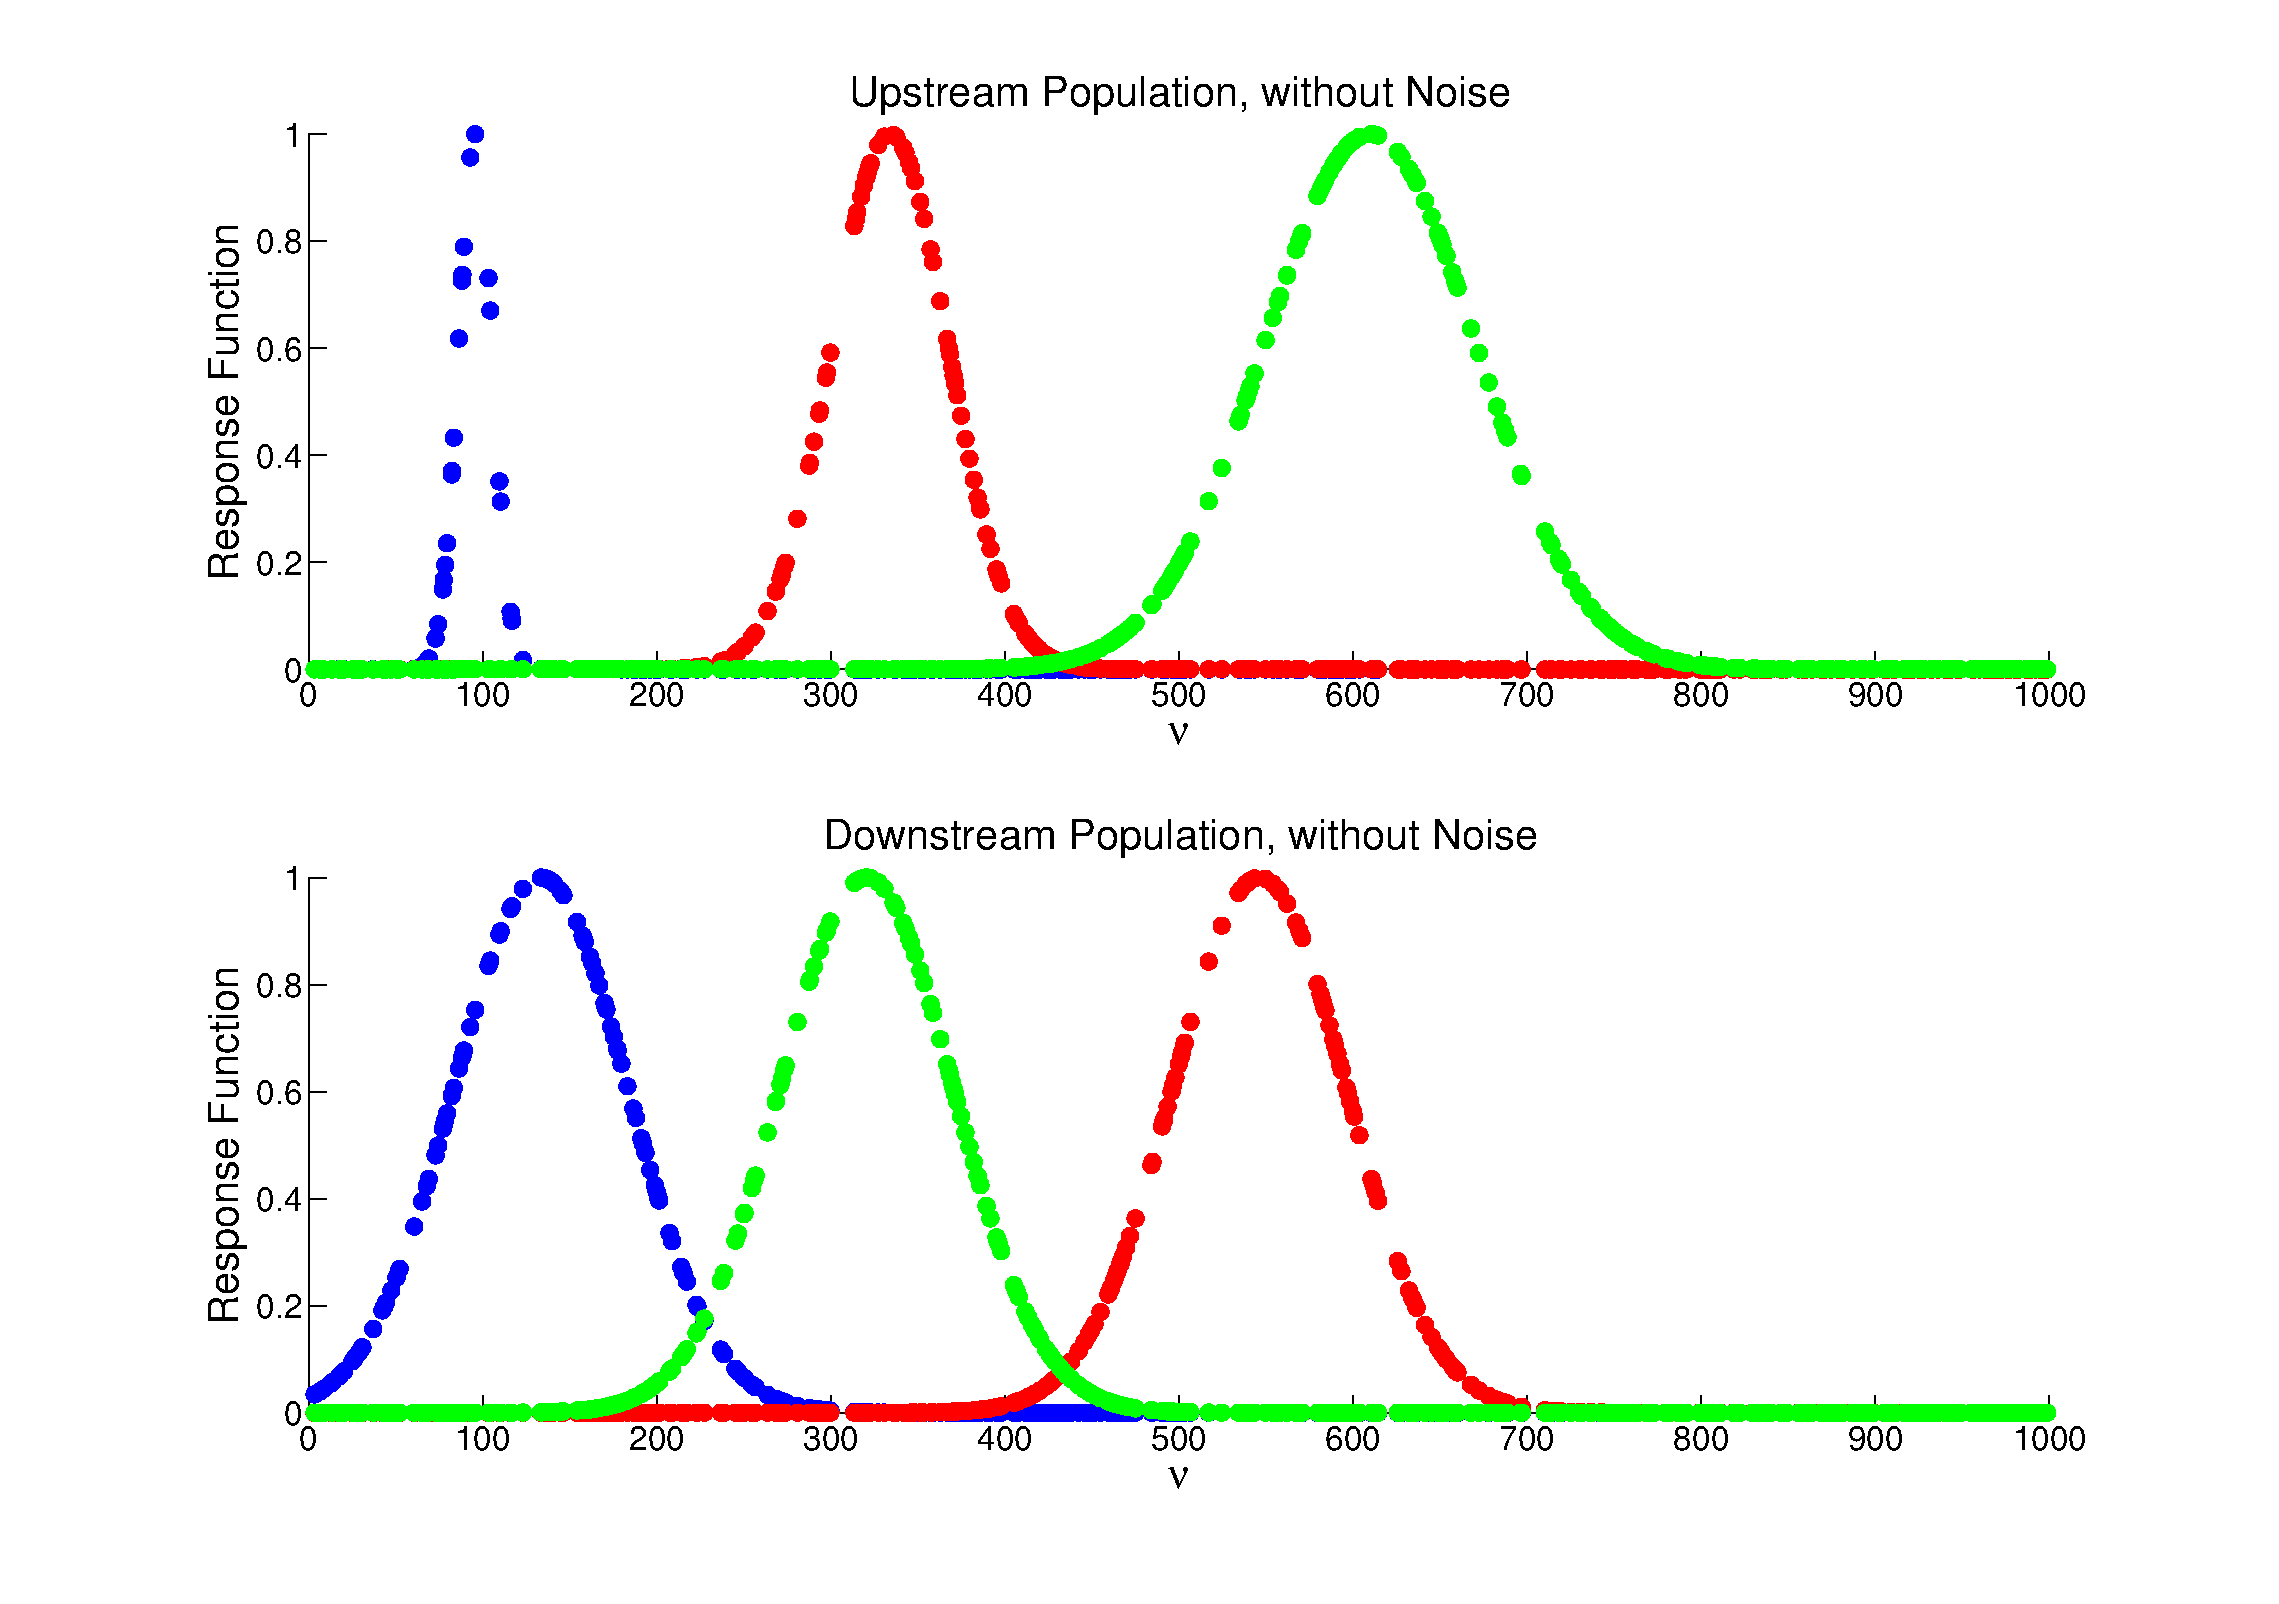
\includegraphics[width=\textwidth, height=80mm]{f1.eps}
% tau4_M1.eps: 0x0 pixel, 300dpi, 0.00x0.00 cm, bb= -304   -42   918   834
\begin{footnotesize}
 Figure 2, Responses of two populations without any noisy $\eta$ factor.
\end{footnotesize}
\end{center}

\begin{center}
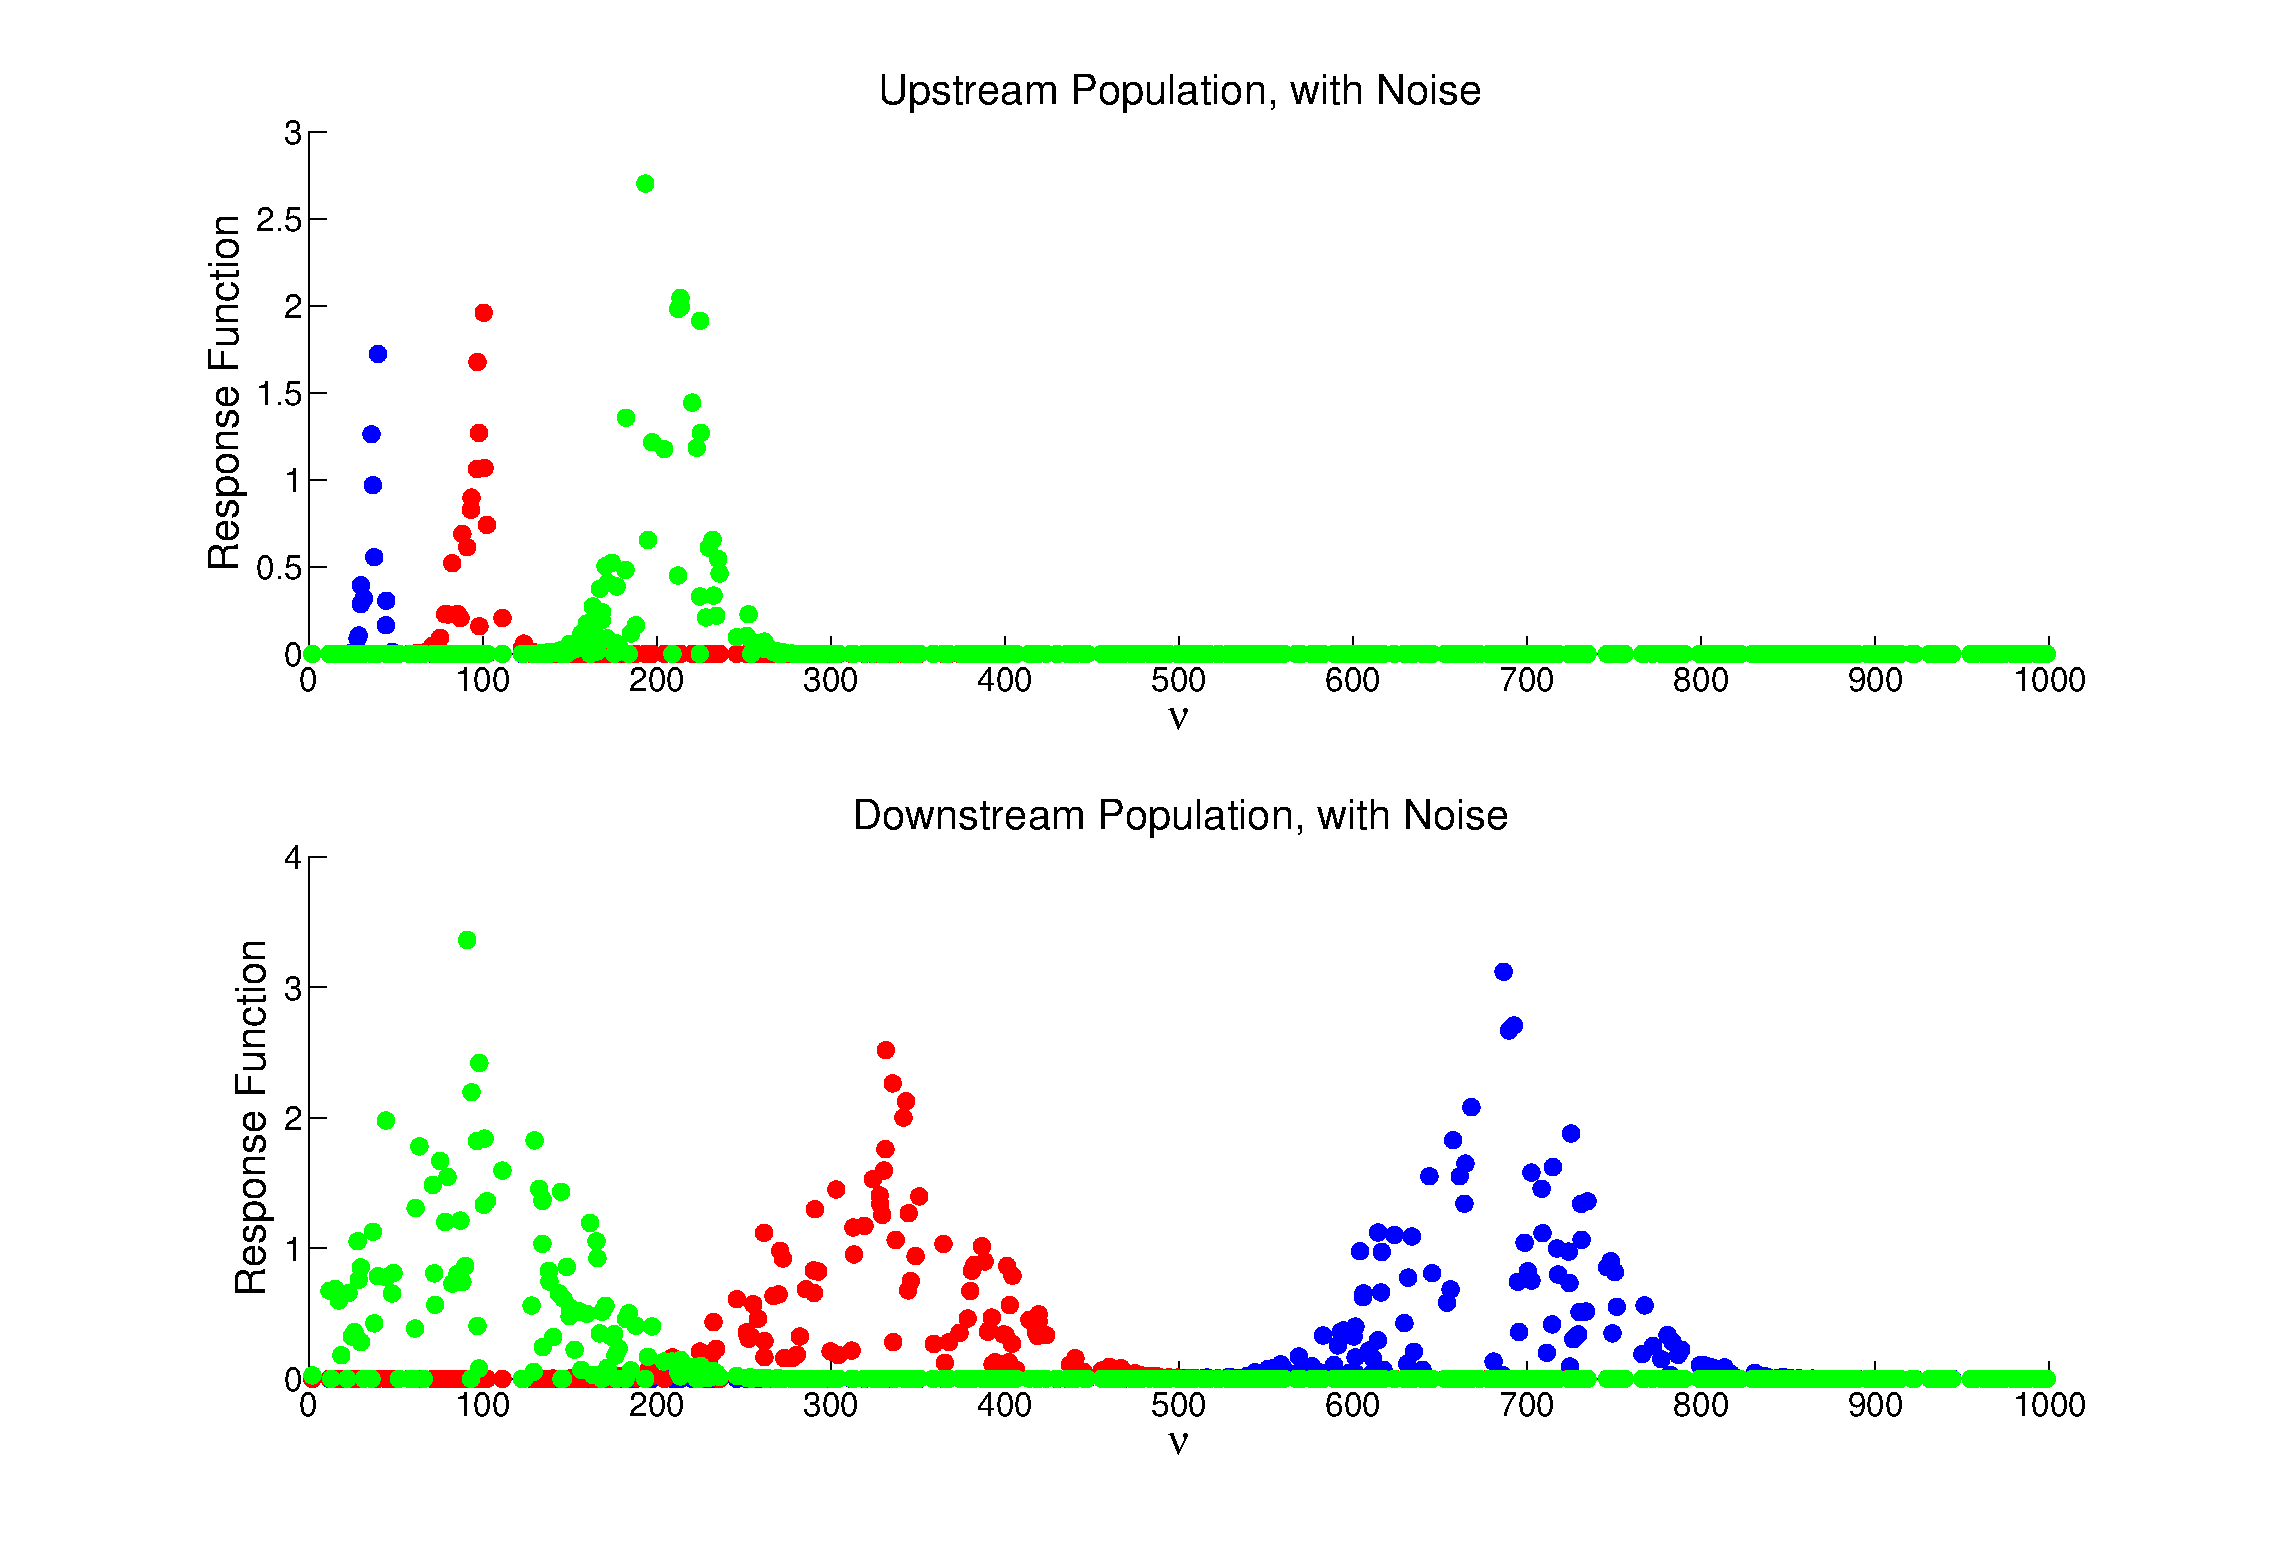
\includegraphics[width=\textwidth,height=80mm]{f2.eps}
% tau4_M1.eps: 0x0 pixel, 300dpi, 0.00x0.00 cm, bb= -304   -42   918   834
\begin{footnotesize}
 Figure 3, Responses of two populations with the noise $\eta$ factor
\end{footnotesize}
\end{center}

Figure 2 and 3 shows the responses of first three neurons from upstream and downstream populations. The responses $R_{L,i}$ and $R_{C,j}$ given by equations 1 and 2 are matrices. Each column of matrices represent the tuning of one neuron e.g. $i$th or $j$th neuron's response is inserted along the $i$th and $j$th column in each response matrix.  

\section{Training of feed-forward connections}
This section starts with the computation of the \textit{covariance matrices}. The covariance for every pair of neurons $ij$ is collected into covariance matrix $W_{ji}$ as the following:

\begin{equation}
 W_{ji}=\langle R_{NL,i} (\nu) R_{L,j}(\nu) \rangle - \langle R_{NL,i}(\nu)\rangle \langle R_{L,j}(\nu) \rangle
\end{equation}

The covariance matrix tells us how the two neuronal networks talk to each other. We assume that each neuron from the first population communicates with other neruons at the second population. The schematic view is shown below.

\begin{center}
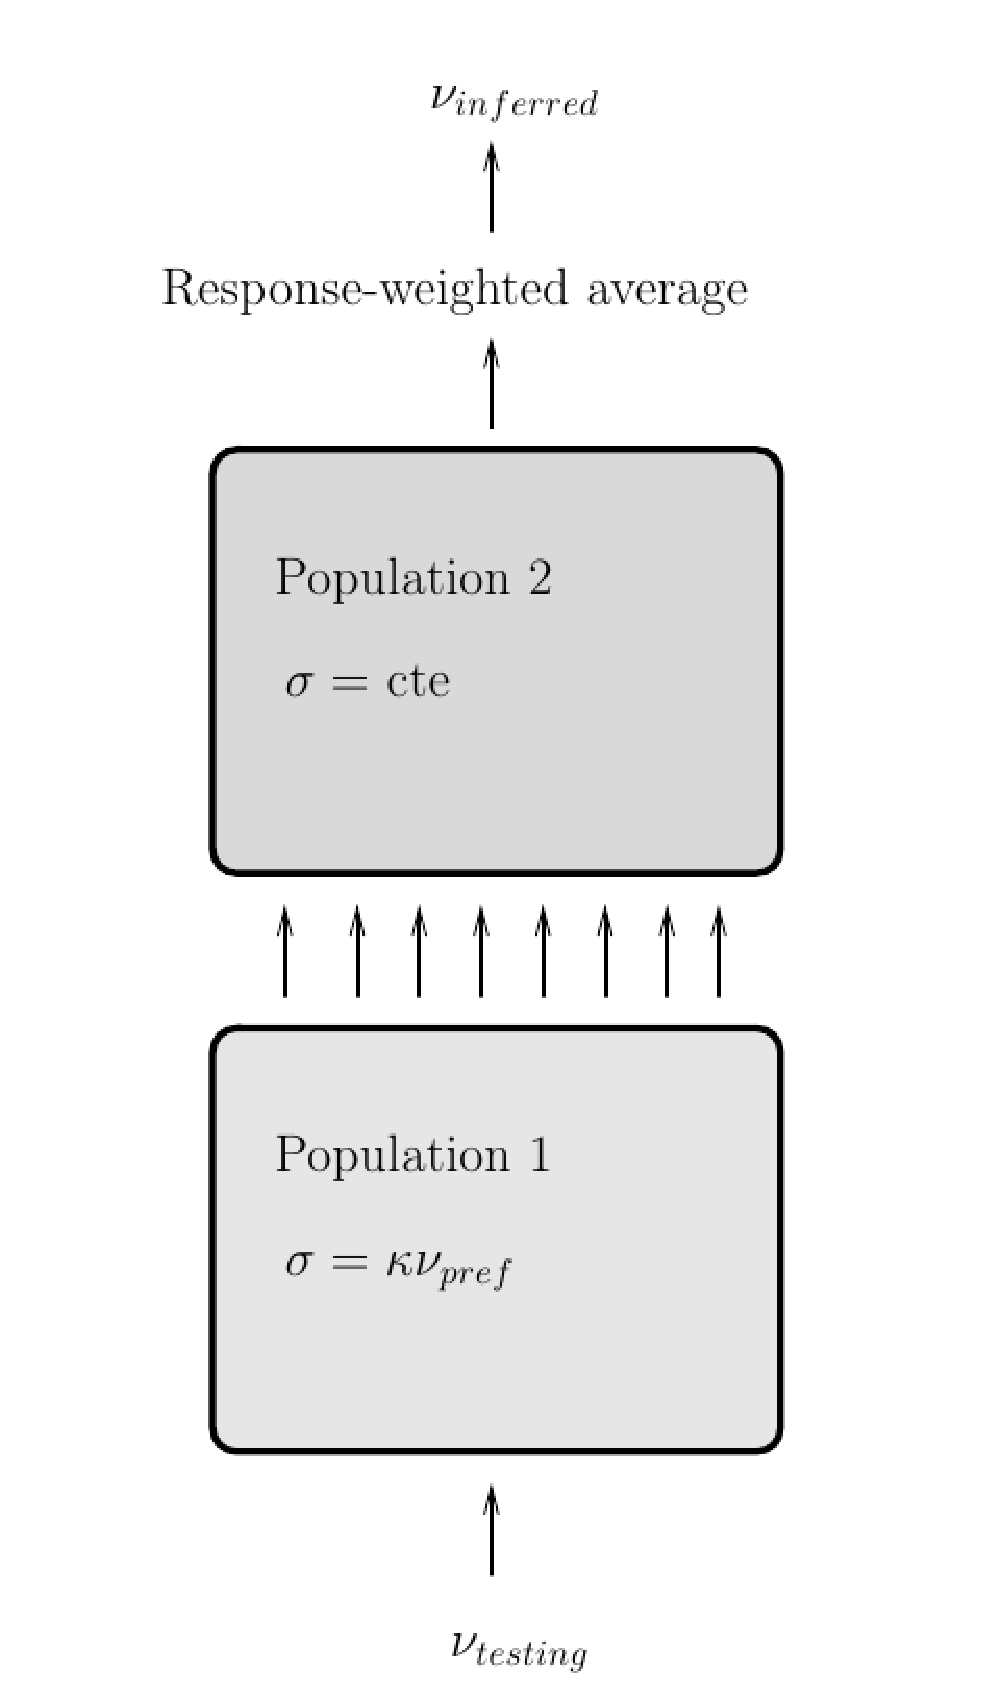
\includegraphics[width=50mm, height=90 mm]{schema2.eps}
% tau4_M1.eps: 0x0 pixel, 300dpi, 0.00x0.00 cm, bb= -304   -42   918   834
\end{center}

\begin{center}
\begin{footnotesize}
 Figure 4, Feedforward connections from upstream population to downstream population
\end{footnotesize}
 \end{center}

\begin{itemize}
 \item Compute the covariance matrices with the provided MATLAB code \textbf{covariance.m} and plot them with the command \textbf{pcolor} for both populations, with or without noise.
\end{itemize}

\begin{center}
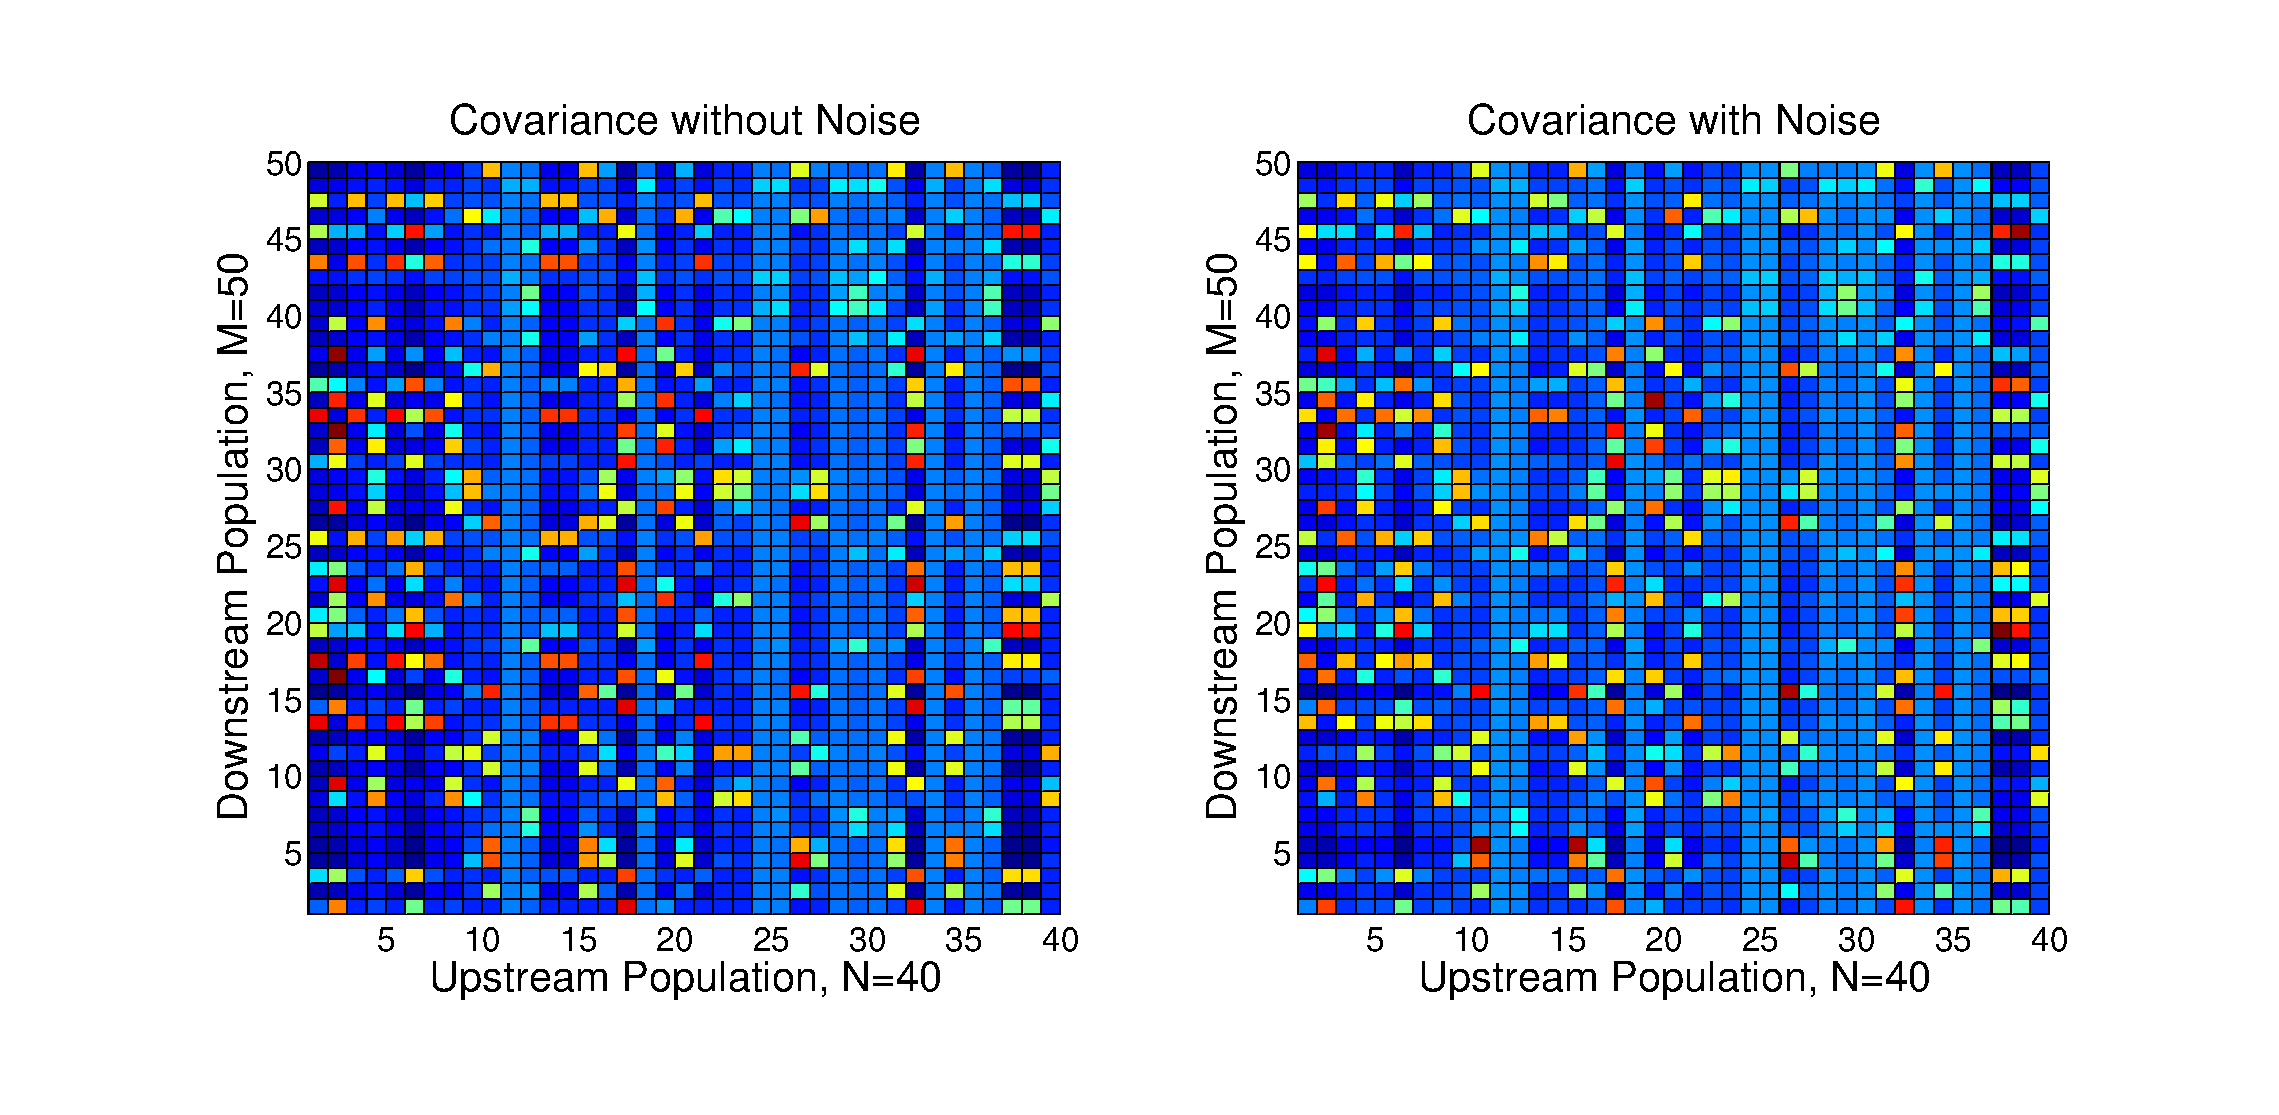
\includegraphics[width=\textwidth, height=80mm]{f3.eps}
% tau4_M1.eps: 0x0 pixel, 300dpi, 0.00x0.00 cm, bb= -304   -42   height=100 mm
\begin{footnotesize}
 Figure 5, Covariance matrices $W_{ji}$ between populations with and without noise factor
\end{footnotesize}
\end{center}

\section{Using feed-forward connections to determine downstream activity}

The downstream population is presumably fed by the upstream population layer with the connectivity matrix $W_{ji}$. The indirect activation of downstream population by the synaptic input from the upstream layer is given by the following equation.

\begin{equation}
 R_{C,j}=(\sum_{i=1}^N W_{ji}\textbf{.}R_{L,i} )_+
\end{equation}

\begin{itemize}
 \item Select new random frequencies $v_{test}$ and as the stimuli and exercise the newly connexted feed-forward network.
\end{itemize}

The provided MATLAB code gives successfully the response of downstream population as stated in equation 4. 

\begin{verbatim}
nu_test=1000*rand(1,12*N);
[r1test_mean r1test_noisy] 
     =GaussResp_LinearSTD(nu_test,nupref_ran1,Rmax,kappa);

r2test_mean=r1test_mean*cov_mean';
r2test_mean(r2test_mean<0)=0;
r2test_noisy=r1test_noisy*cov_noisy';

\end{verbatim}

\section{Decoding the downstream activity}
This task aims to "decode" the downstream activity. We assume that, we see the output $R_{C,j}$ of the downstream population and we know the preffered frequency of each neuron from the same population $v_{pref,C,j}$. How to guess the input driving frequency so called $v_{inferred}$? The answer is to compute the response-weighted average of the preferred frequencies as the following:

\begin{equation}
 v_{inferred}=\dfrac{\sum_{j=1} ^M R_{C,j} v_{pref,C,j}}{\sum_{j=1} ^M R_{C,j}}
\end{equation}

\begin{itemize}
 \item Plot $v_{test}$ versus $v_{inferred}$
\end{itemize}

\begin{center}
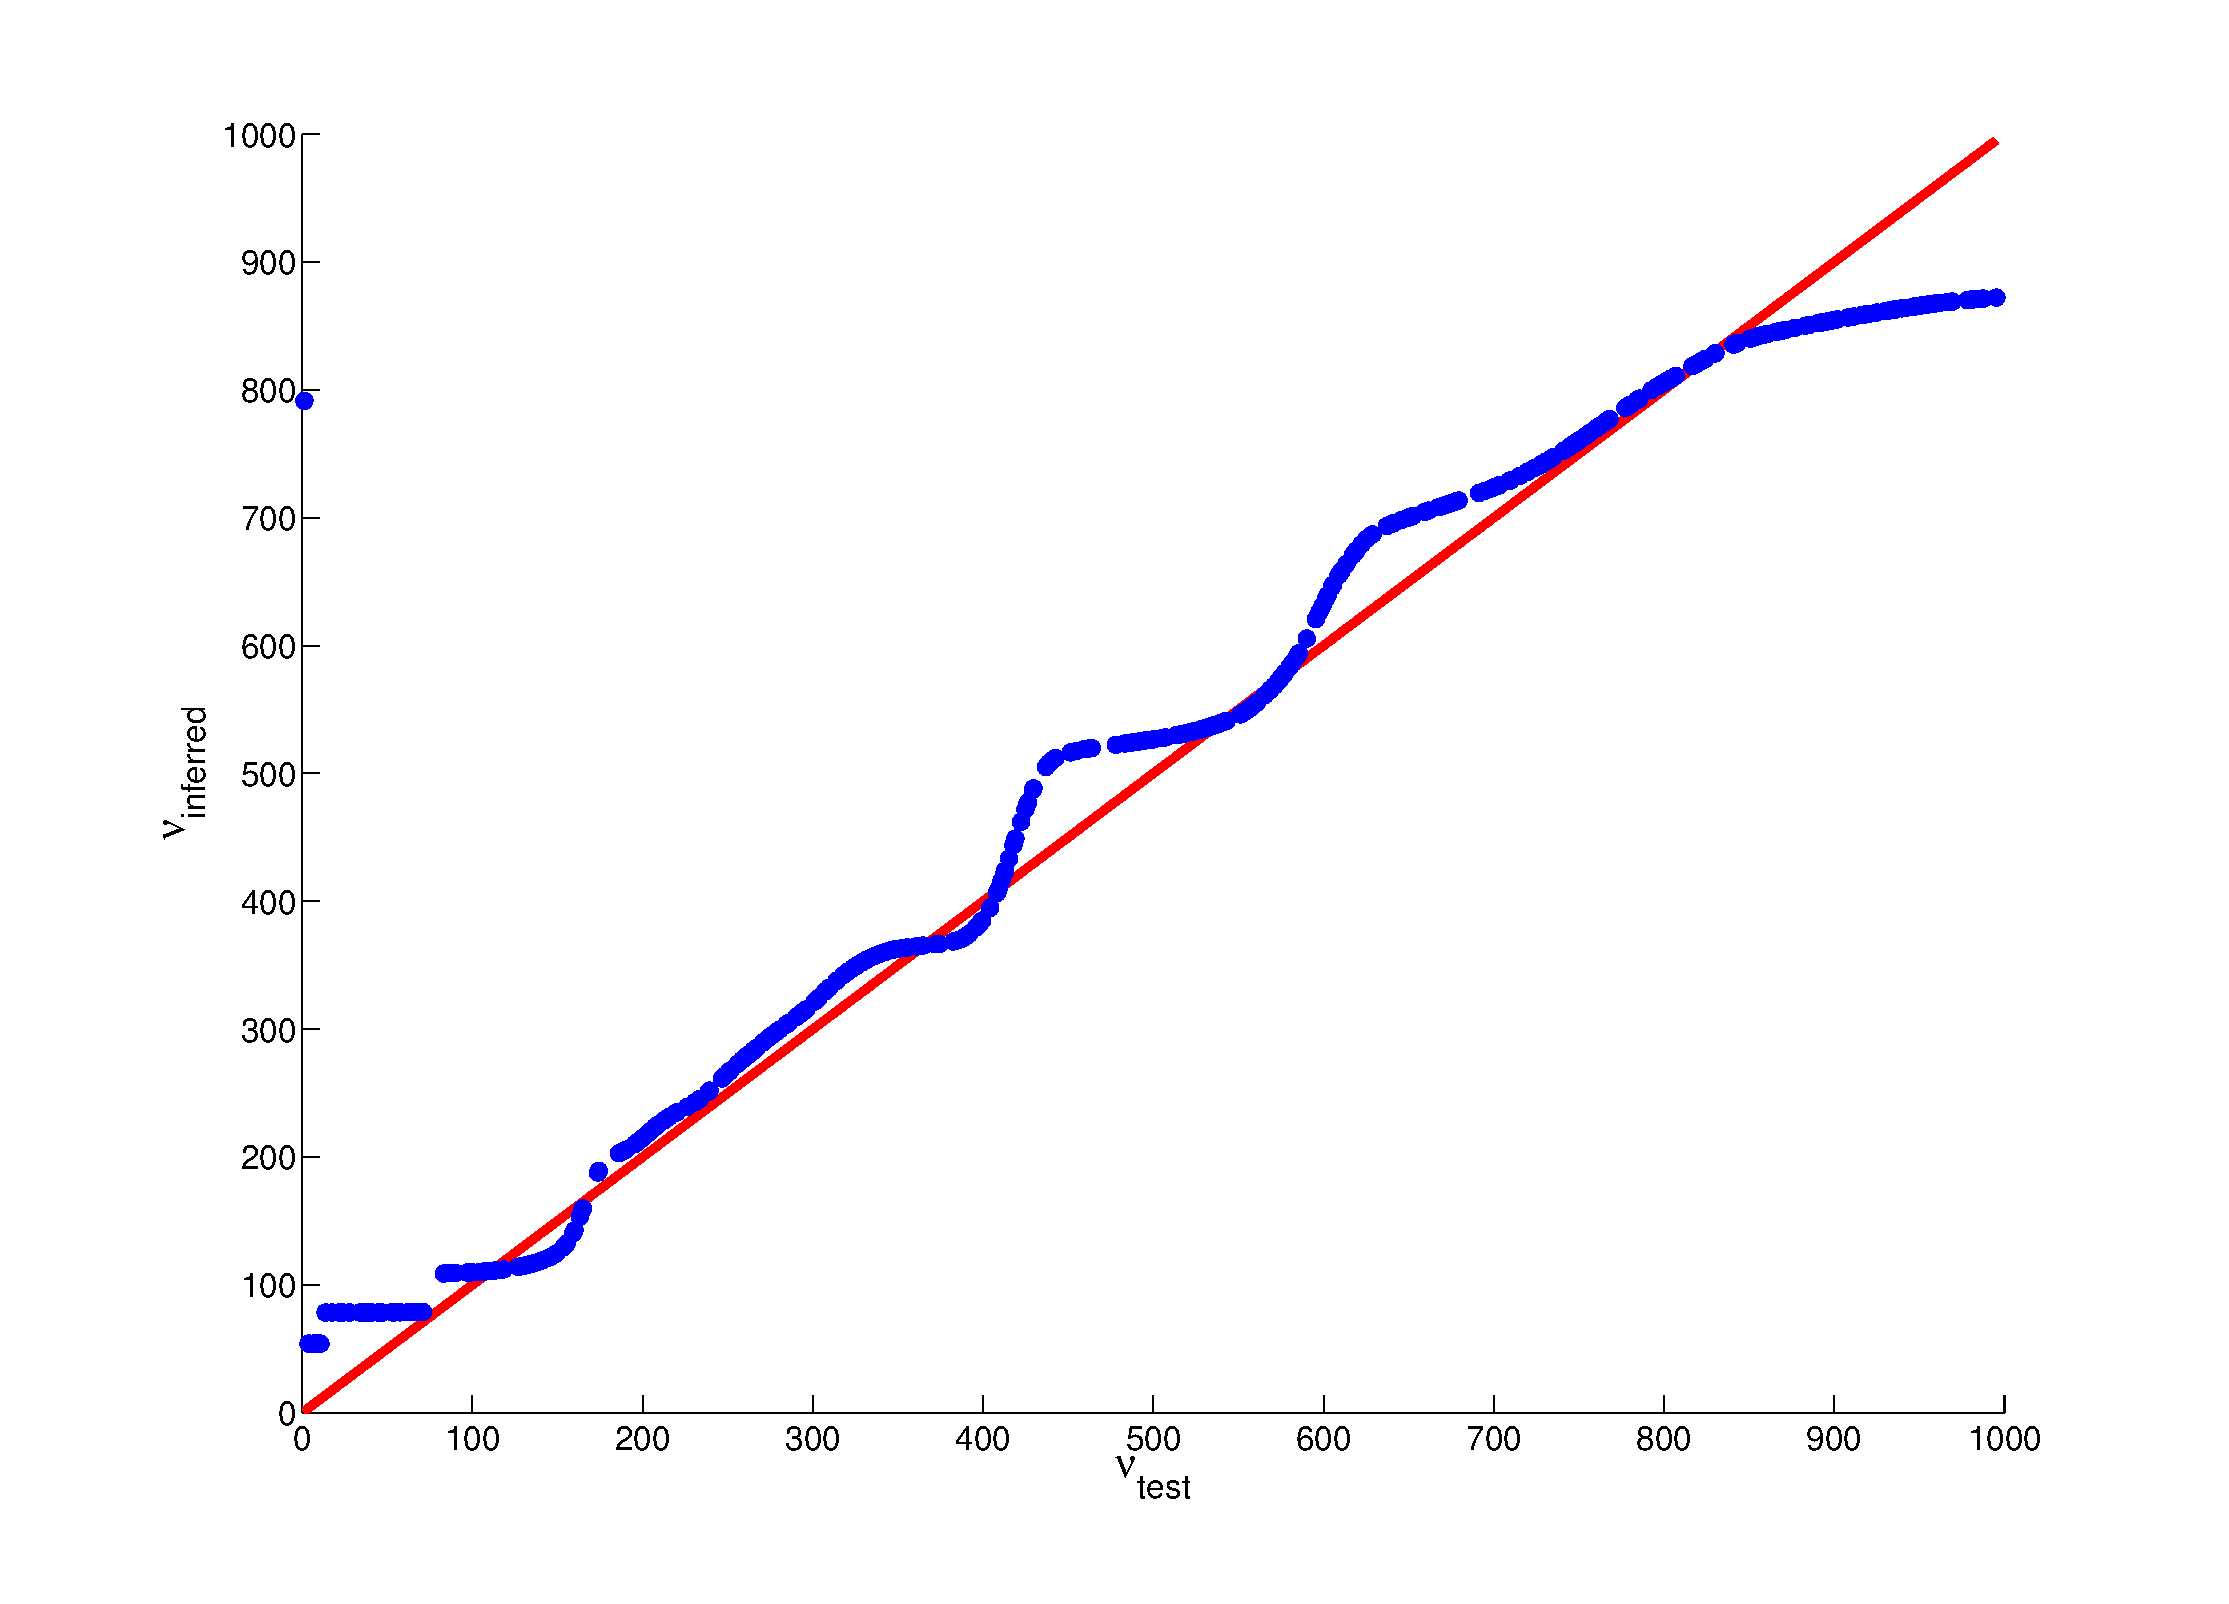
\includegraphics[width=\textwidth, height=80mm]{f4.eps}
% tau4_M1.eps: 0x0 pixel, 300dpi, 0.00x0.00 cm, bb= -304   -42   height=100 mm
\begin{footnotesize}
 Figure 6, comparison of $v_{test}$ and $v_{inferred}$. They seem to be quite good fitting
\end{footnotesize}
\end{center}

\begin{itemize}
 \item Discuss the effect of $\kappa$, $\sigma$ and total number of neurons M and N in each population on the Figure 6.
\end{itemize}

Let us increase $\kappa$ from 0.1 to 1 and have a look at covariance matrices between two populations and also observe the change in Figure 6. 

\begin{center}
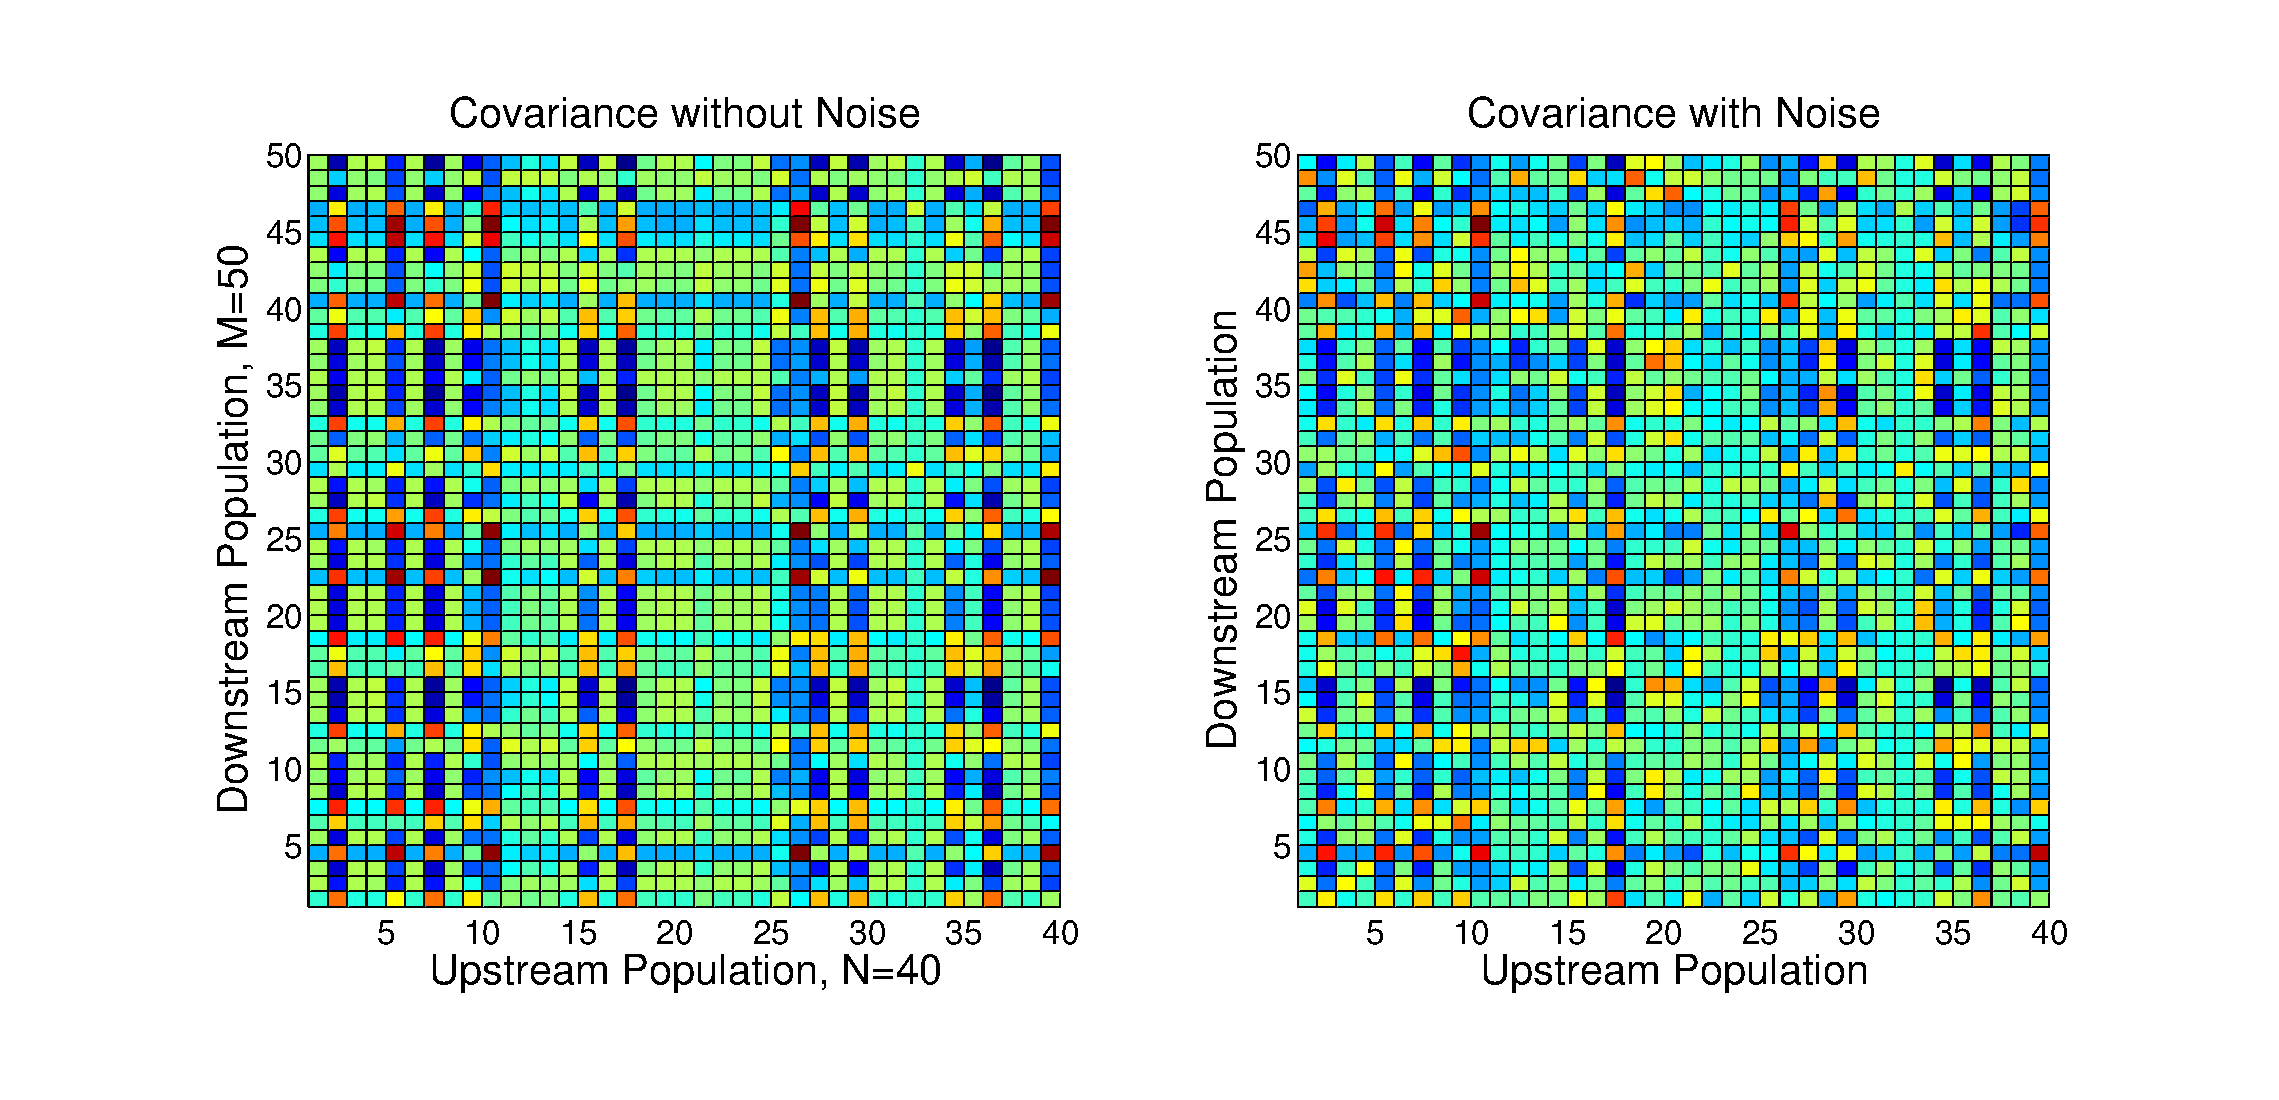
\includegraphics[width=\textwidth]{kappa2.eps}
% tau4_M1.eps: 0x0 pixel, 300dpi, 0.00x0.00 cm, bb= -304   -42   height=100 mm
\begin{footnotesize}
 Figure 7, $\kappa=1$
\end{footnotesize}
\end{center}

\begin{center}
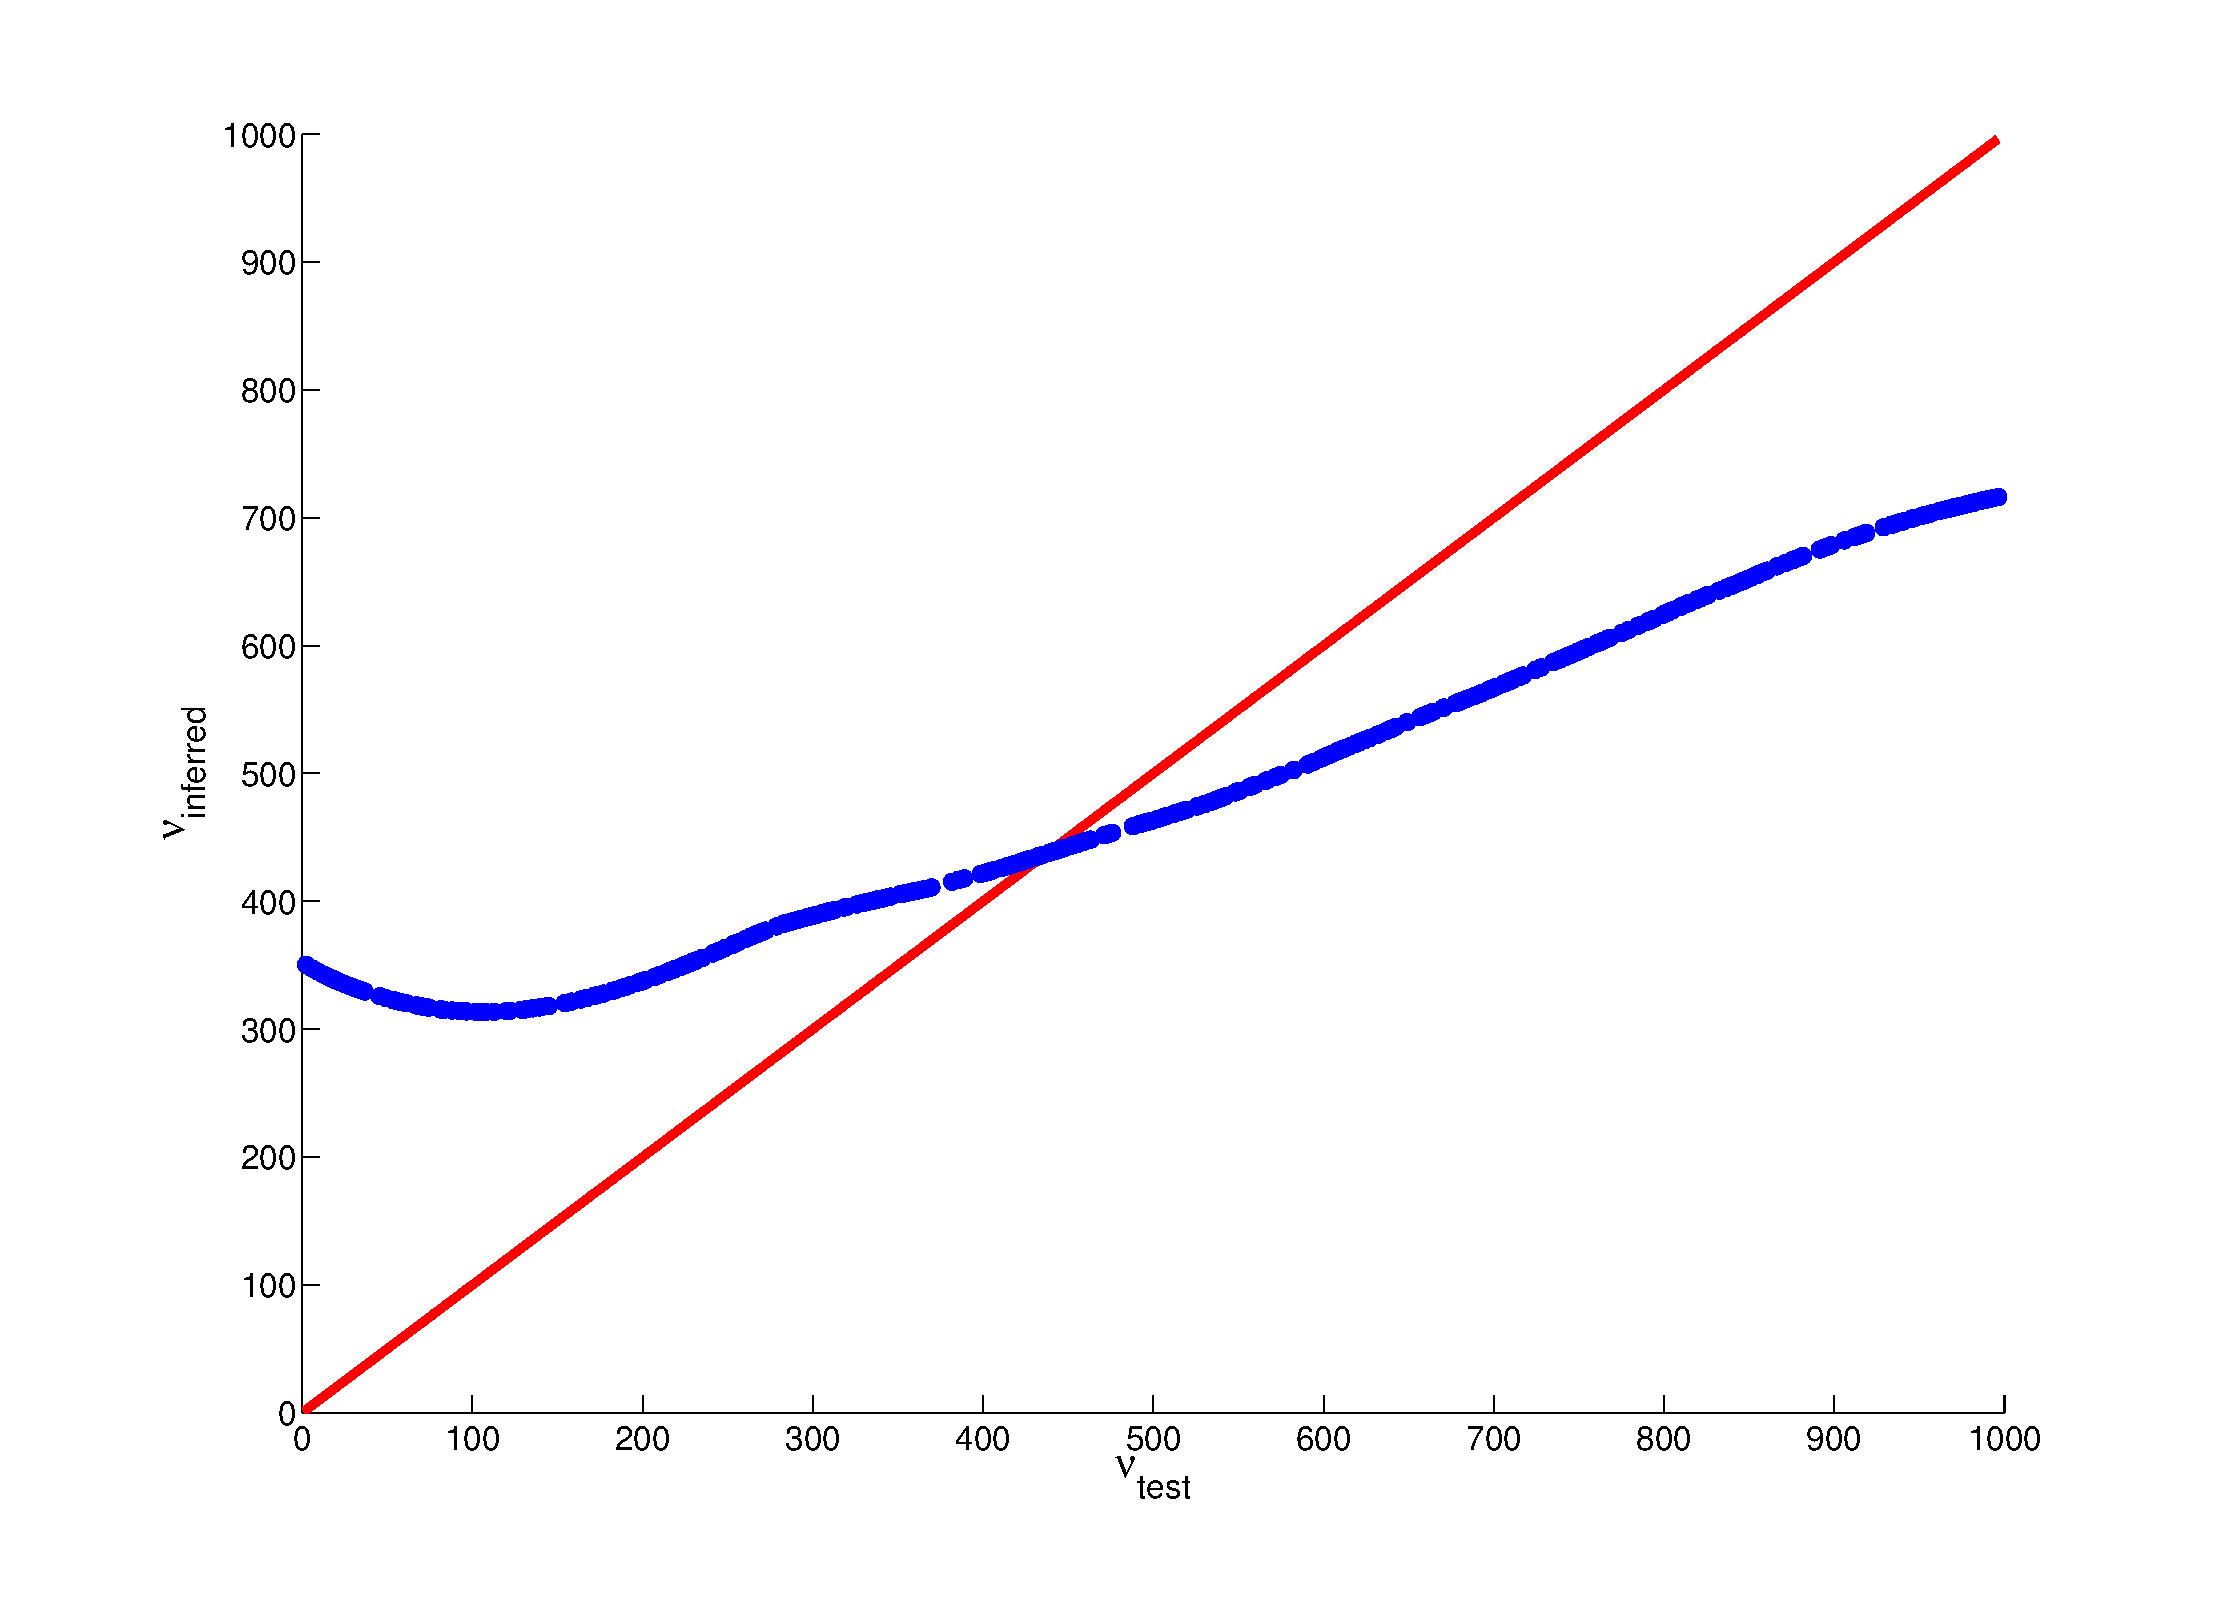
\includegraphics[width=\textwidth]{kappa.eps}
% tau4_M1.eps: 0x0 pixel, 300dpi, 0.00x0.00 cm, bb= -304   -42   height=100 mm
\begin{footnotesize}
 Figure 8, $\kappa=1$
\end{footnotesize}
\end{center}

Obvioulsy $v_{inferred}$ does not fit to $v_{test}$ now as it was before in Figure 6. This is due to the change in covariance matrices. Figure 7 shows the new cowariance matrices between two populations. The color distribution is relatively different than Figure 5, it means the two populations cannot communicate ``well'' now, so the input frequency decoding is not really satisfactory. So $\kappa$ is an highly effective factor on communication of two populations. 

Let us increase the $\sigma$ from 50 to 100 and observe its effects.

\begin{center}
\includegraphics[width=\textwidth]{sigma_big1.eps}
% tau4_M1.eps: 0x0 pixel, 300dpi, 0.00x0.00 cm, bb= -304   -42   height=100 mm
\begin{footnotesize}
 Figure 9, $\sigma=100$
\end{footnotesize}
\end{center}

\begin{center}
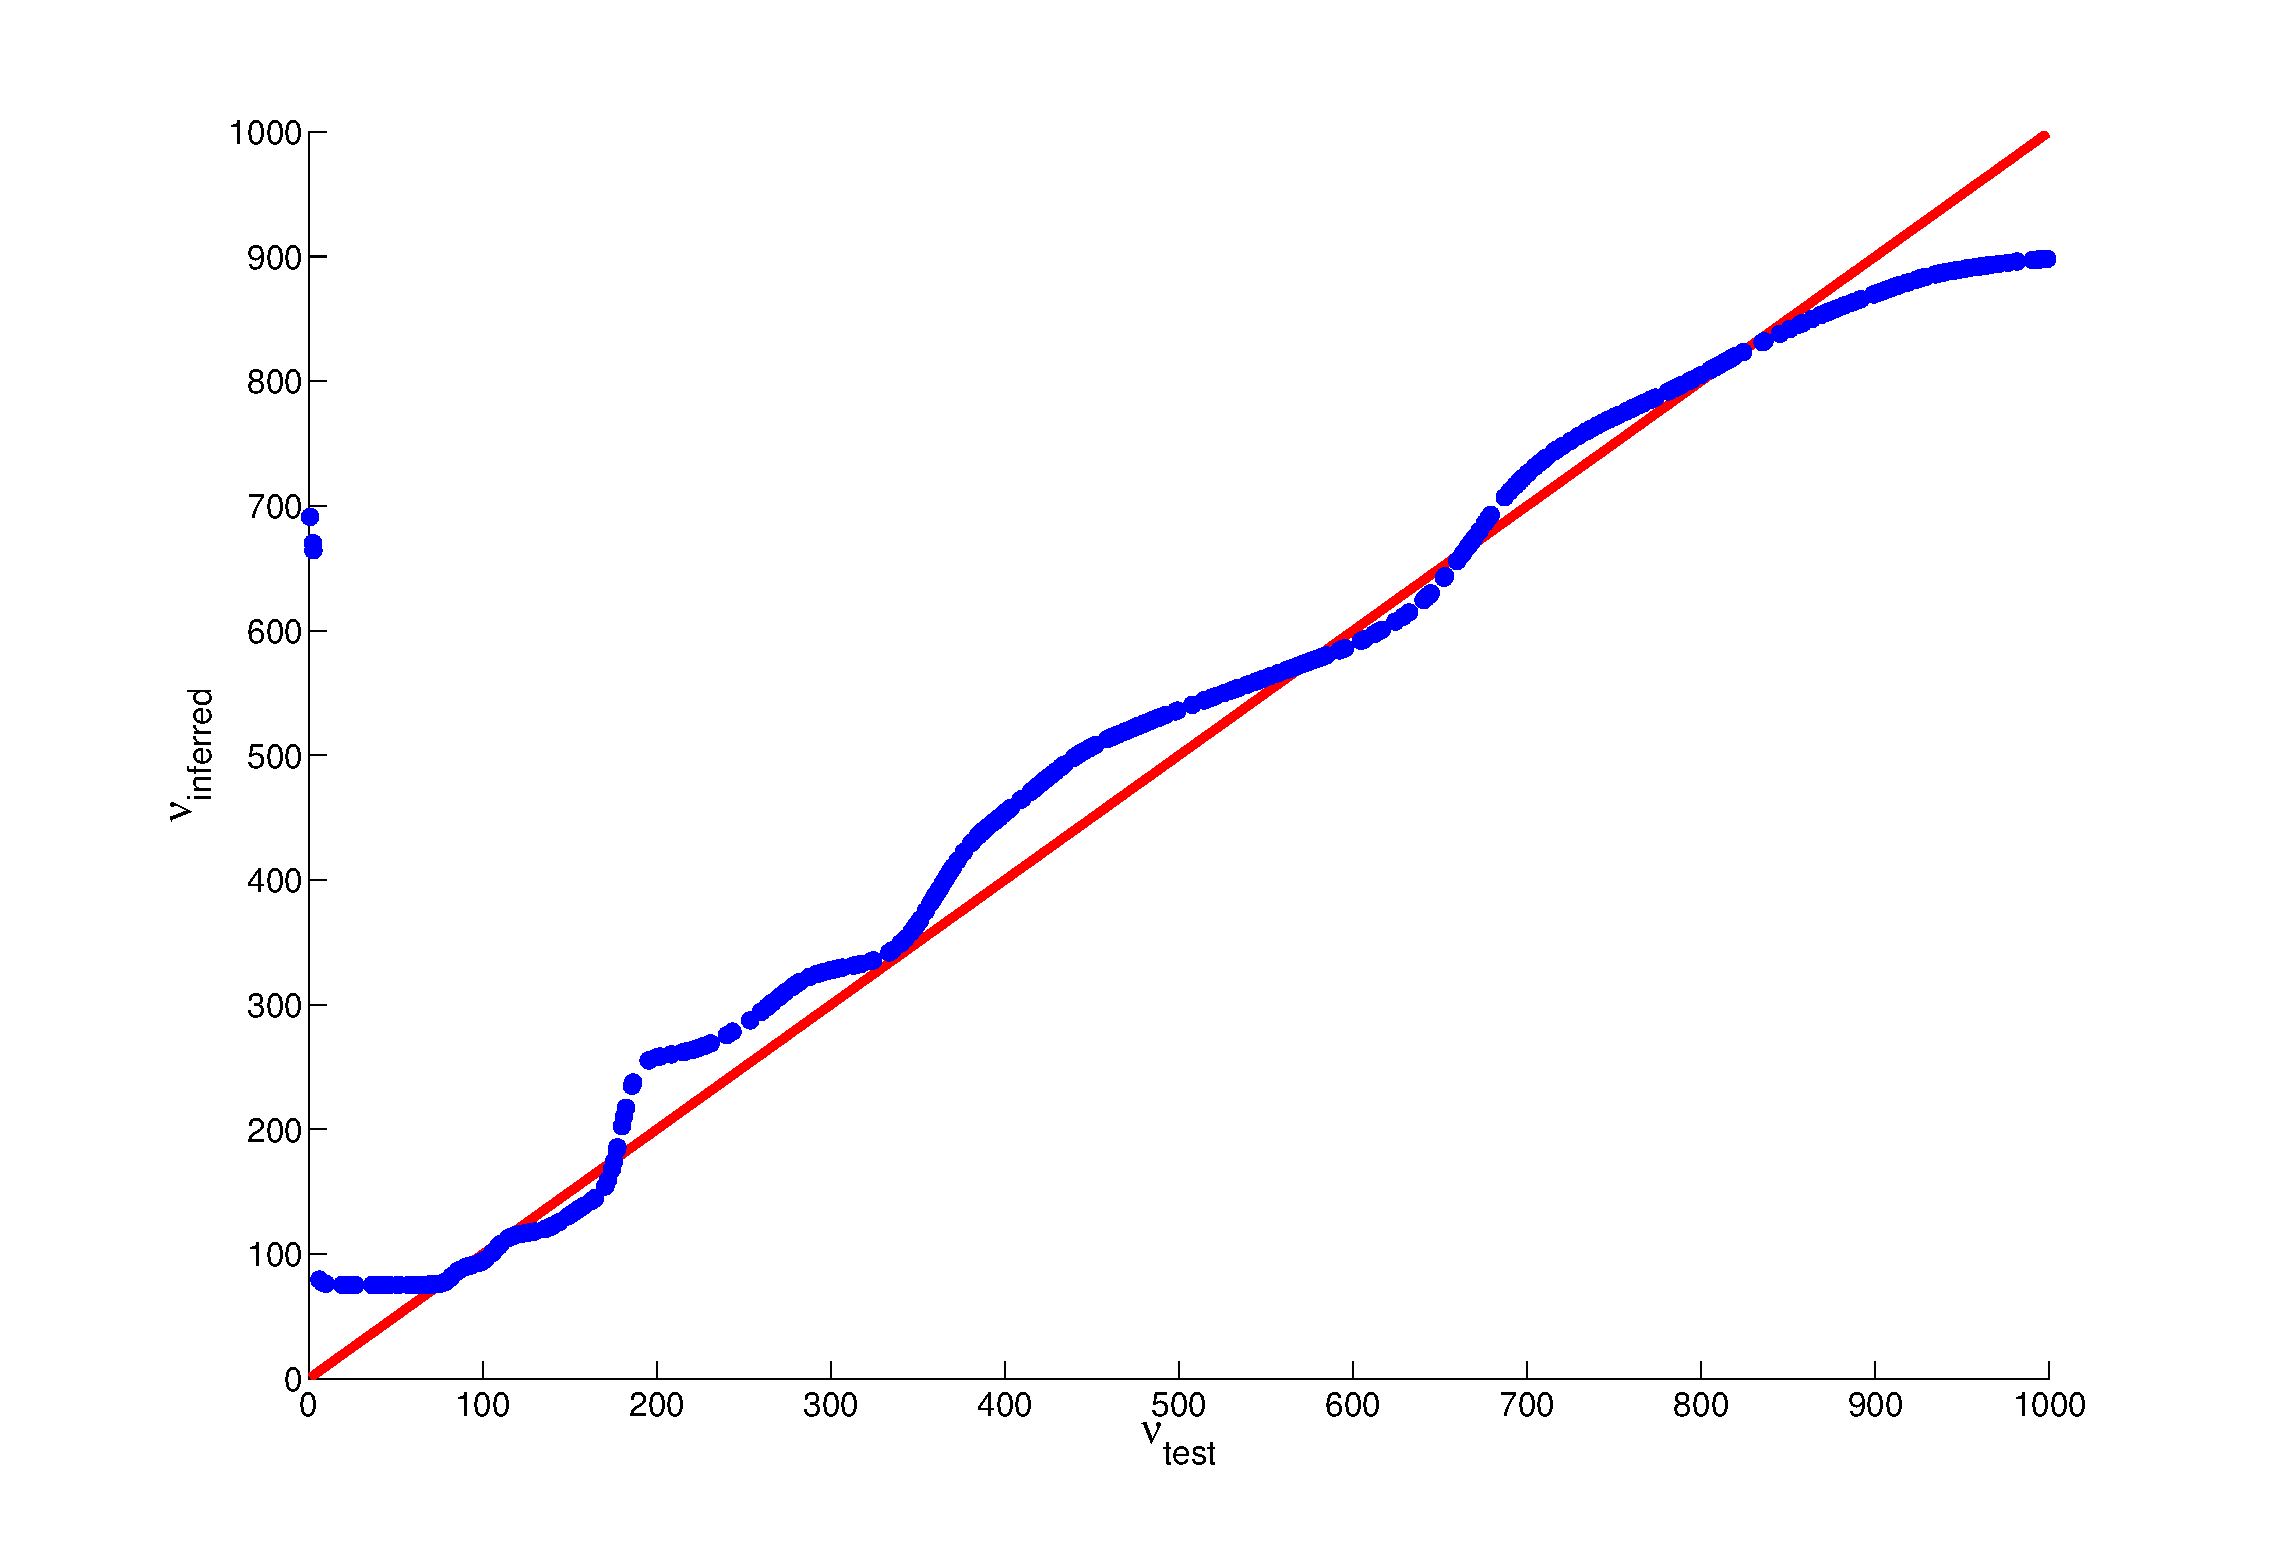
\includegraphics[width=\textwidth]{sigma_big2.eps}
% tau4_M1.eps: 0x0 pixel, 300dpi, 0.00x0.00 cm, bb= -304   -42   height=100 mm
\begin{footnotesize}
 Figure 10, $\sigma=100$
\end{footnotesize}
\end{center}

$\sigma$ represents the standard deviation in Gaussian distributed noisy part stated by equations 1 and 2 before. Therefore it is expected the width of the neuronal tuning graphs increase. This is easily seen when Figure 9 is compared to Figure 2. However, Figure 10 is not clearly different from Figure 6, decoding is not strongly affected. The same procedures were repeated for a very small $\sigma$ value, e.g. 1. This time the width of neuronal tunings on noisy graphs reduced, decoding was again not really affected. 

Now, let us change number of neurons M and N to bigger values.

\begin{center}
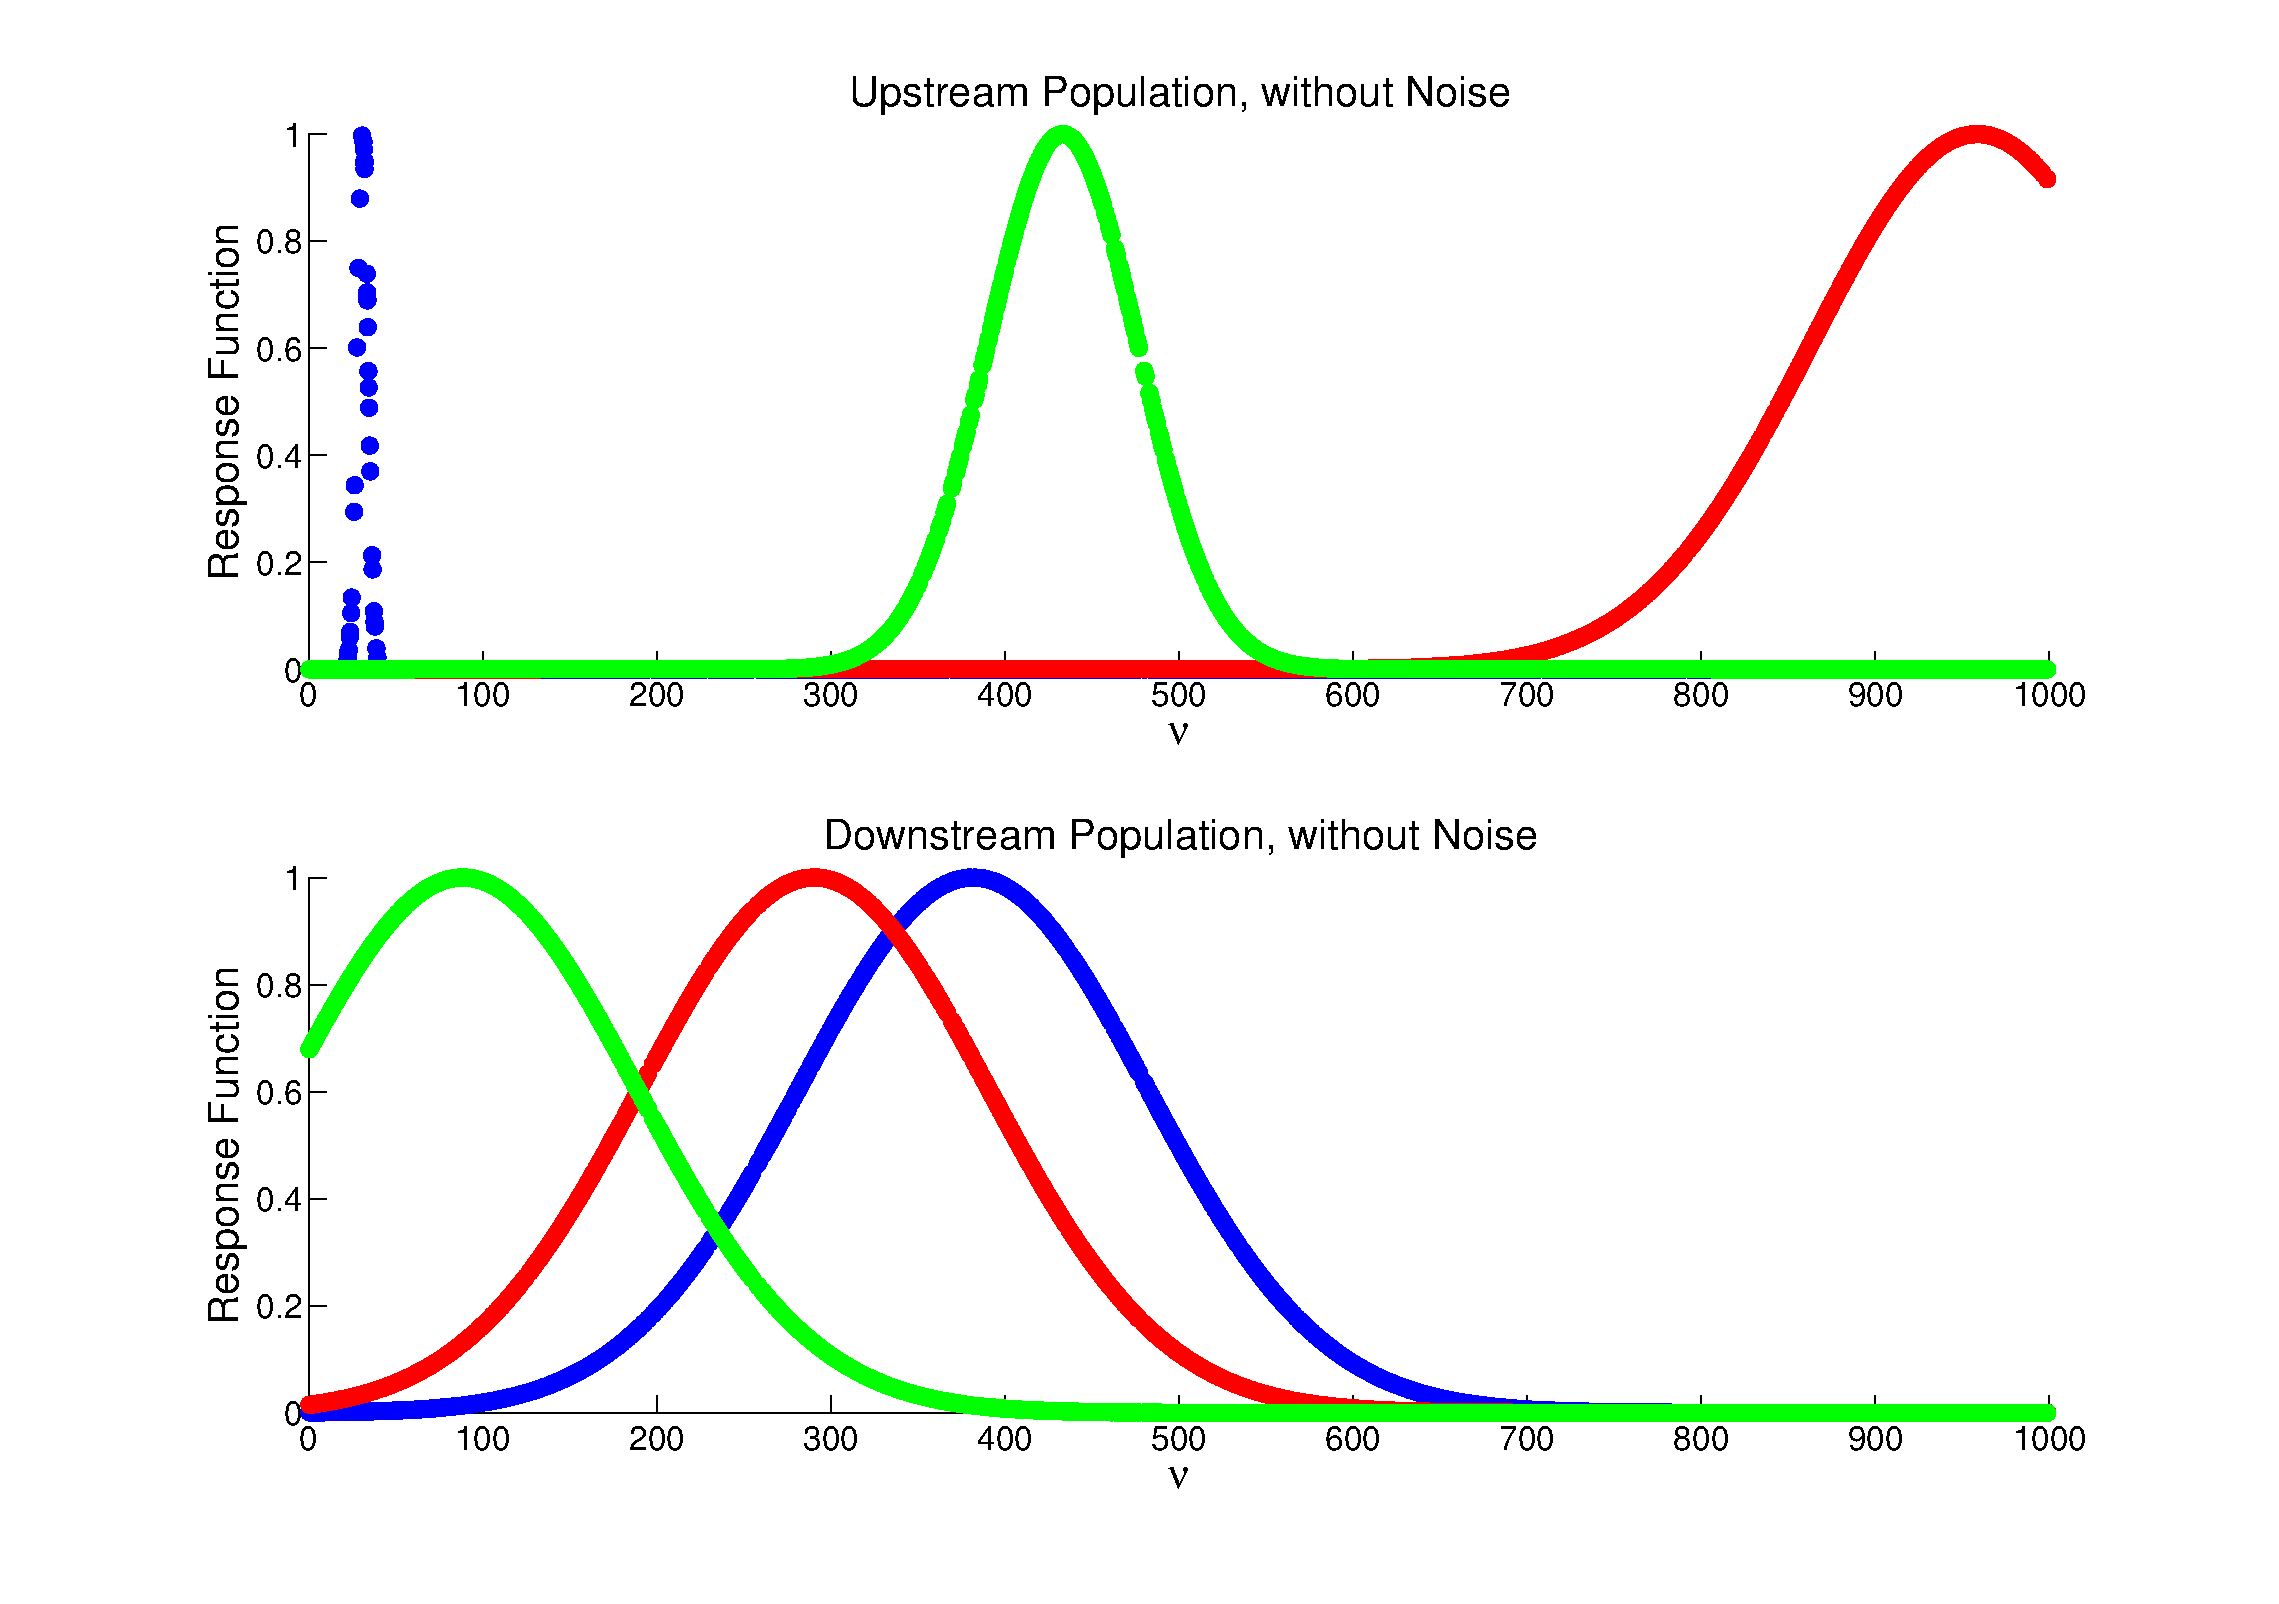
\includegraphics[width=\textwidth]{MN_big1.eps}
% tau4_M1.eps: 0x0 pixel, 300dpi, 0.00x0.00 cm, bb= -304   -42   height=100 mm
\begin{footnotesize}
 Figure 11, $M=200$, $N=200$
\end{footnotesize}
\end{center}


\begin{center}
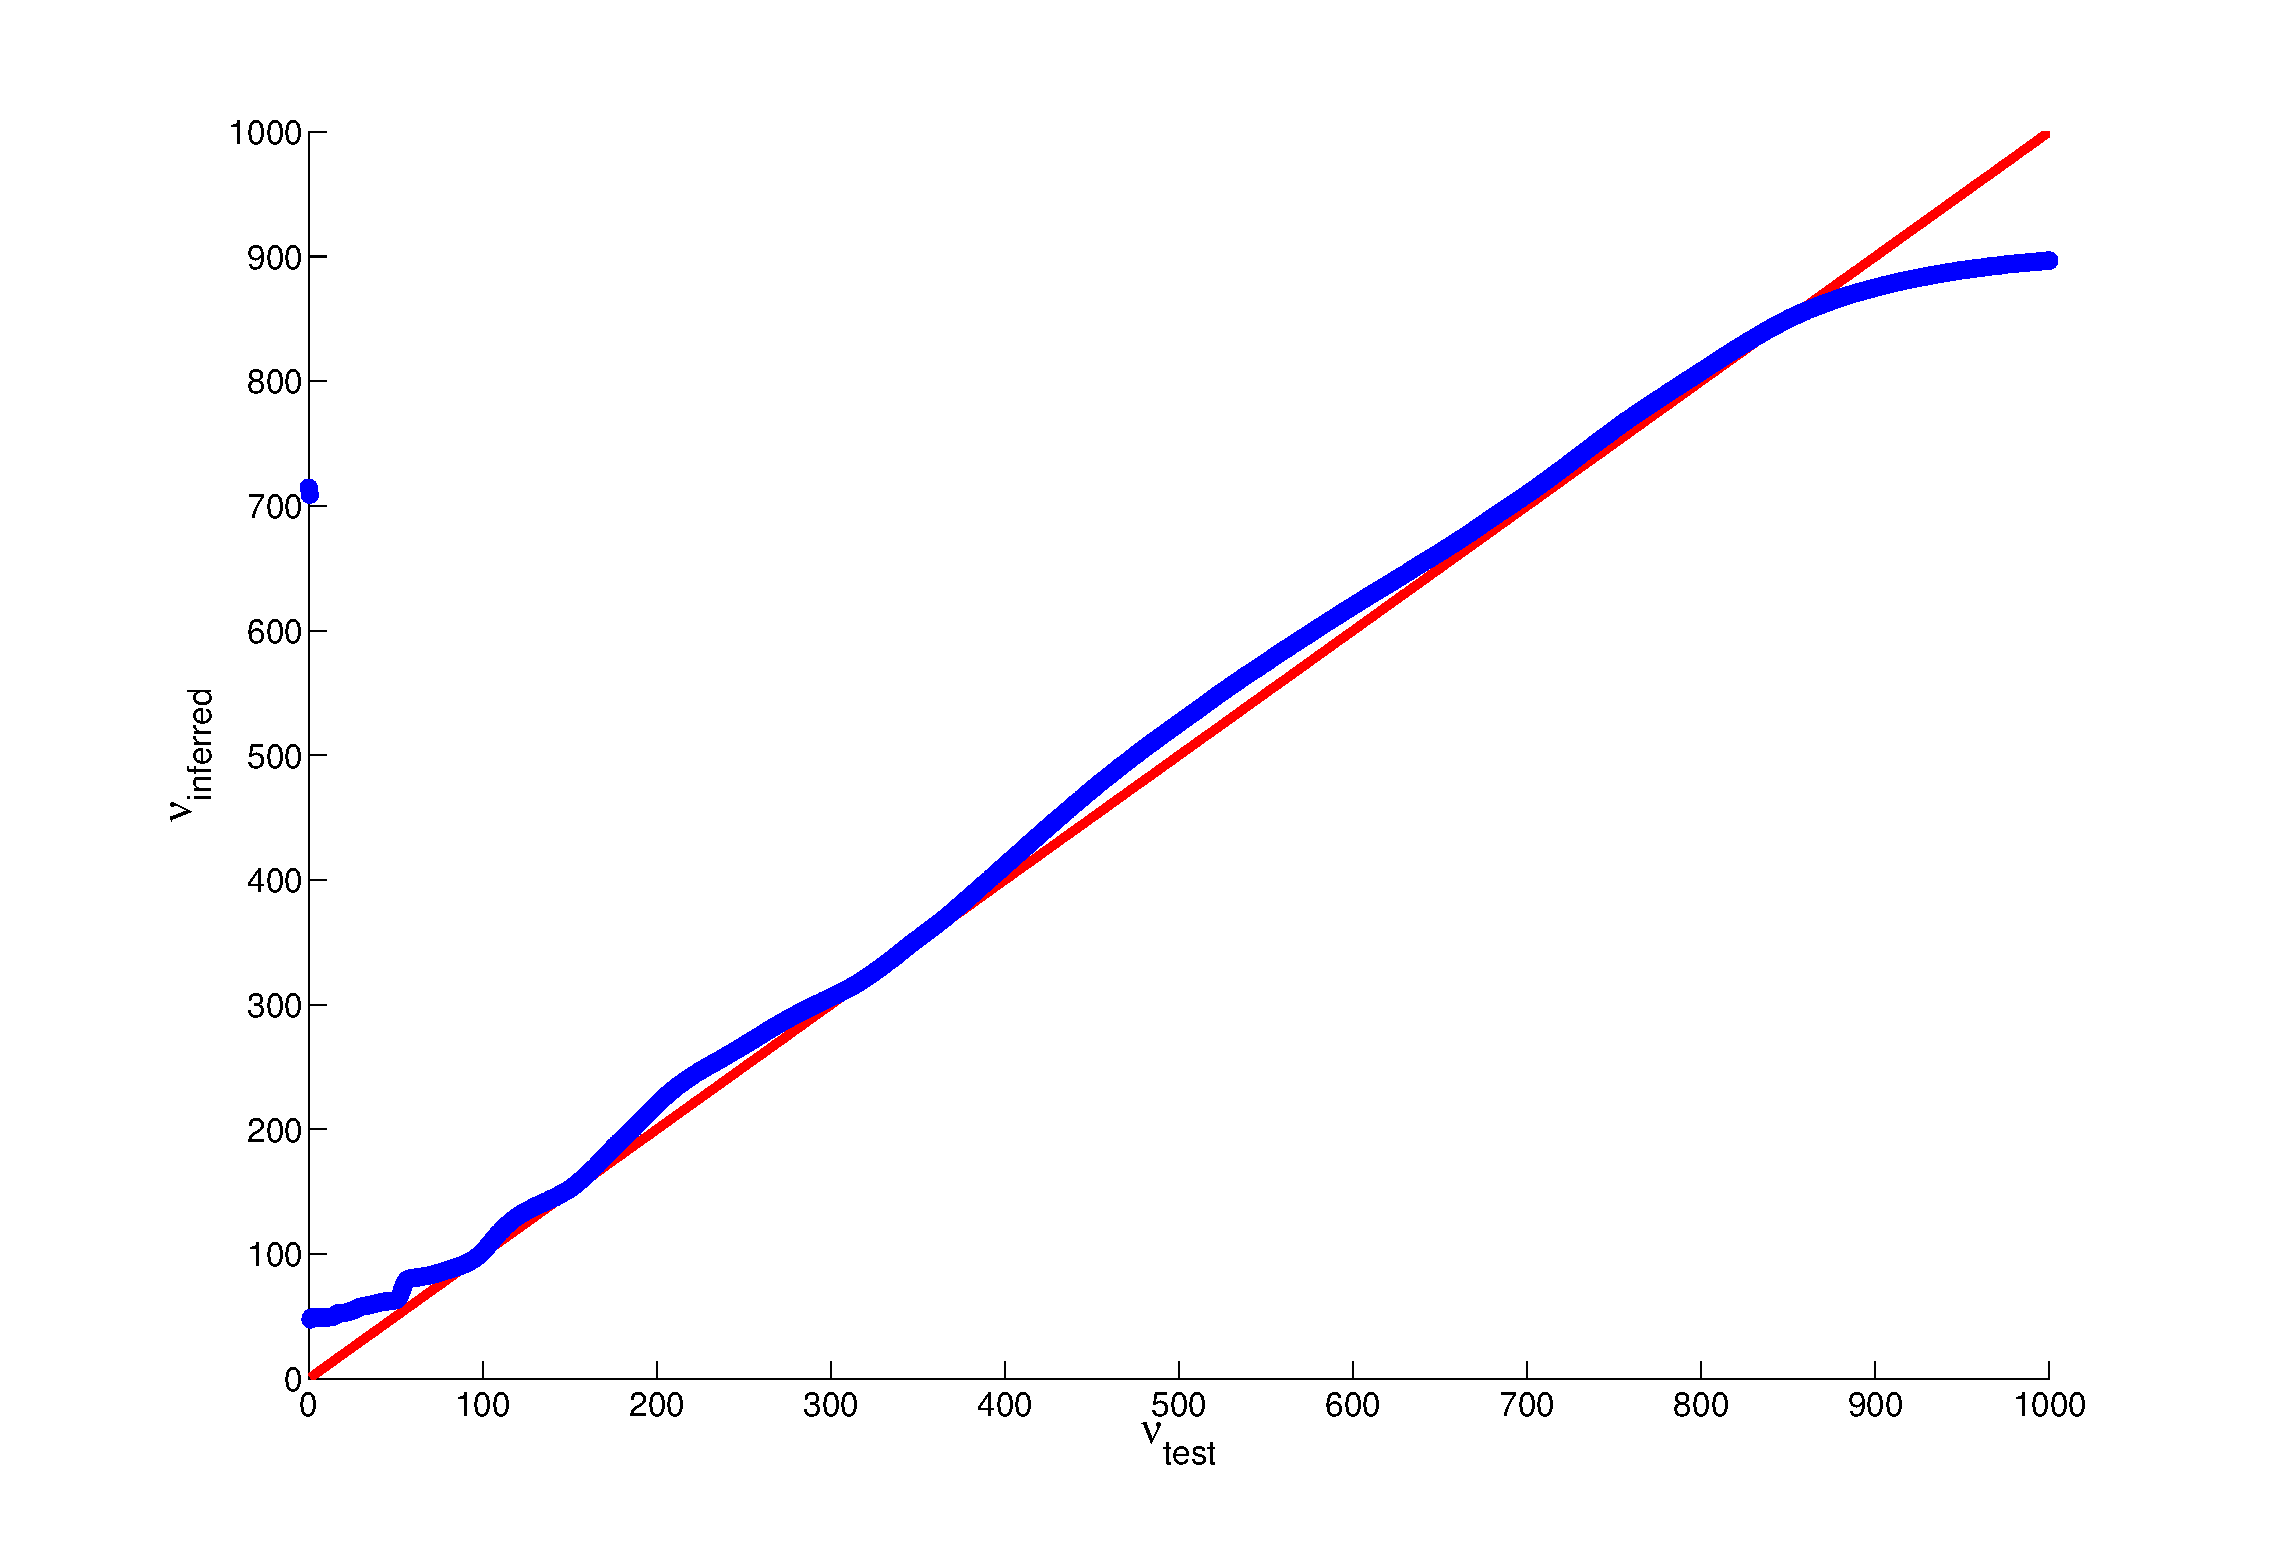
\includegraphics[width=\textwidth, height=70mm]{MN_big2.eps}
% tau4_M1.eps: 0x0 pixel, 300dpi, 0.00x0.00 cm, bb= -304   -42   height=100 mm
\begin{footnotesize}
 Figure 12, $M=200$, $N=200$
\end{footnotesize}
\end{center}

The more neurons there exist in each population, the bigger communication network is built. The tuning of the neurons become more clear to observe in Figure 11 in comparison to Figure 2. This can be thought as the following: The dimensions of the response matrix become larger in both columns and rows. Now, for each neuron there exist many data points to be plotted in their tuning curves. It might be also said, the tuning of curves overlap more with incresing neuron numbers as seen in downstream population withouth noise graph on figure 11.

Not only the response matrices, but also the covariance matrices seem to grow large. All the other parameters are fixed e.g. $\kappa$ and $\sigma$ to their previous values except for M and N values. Since there are more neurons communicating now, we expect to guess the input frequency $v_{inferred}$ more precisely. Figure 12 approves this expectation. $v_{inferred}$ fits better this time to $v_{test}$ in comparison to Figure 6.


What happens if M and N are reduced e.g. to 15 and 10? 
\begin{center}
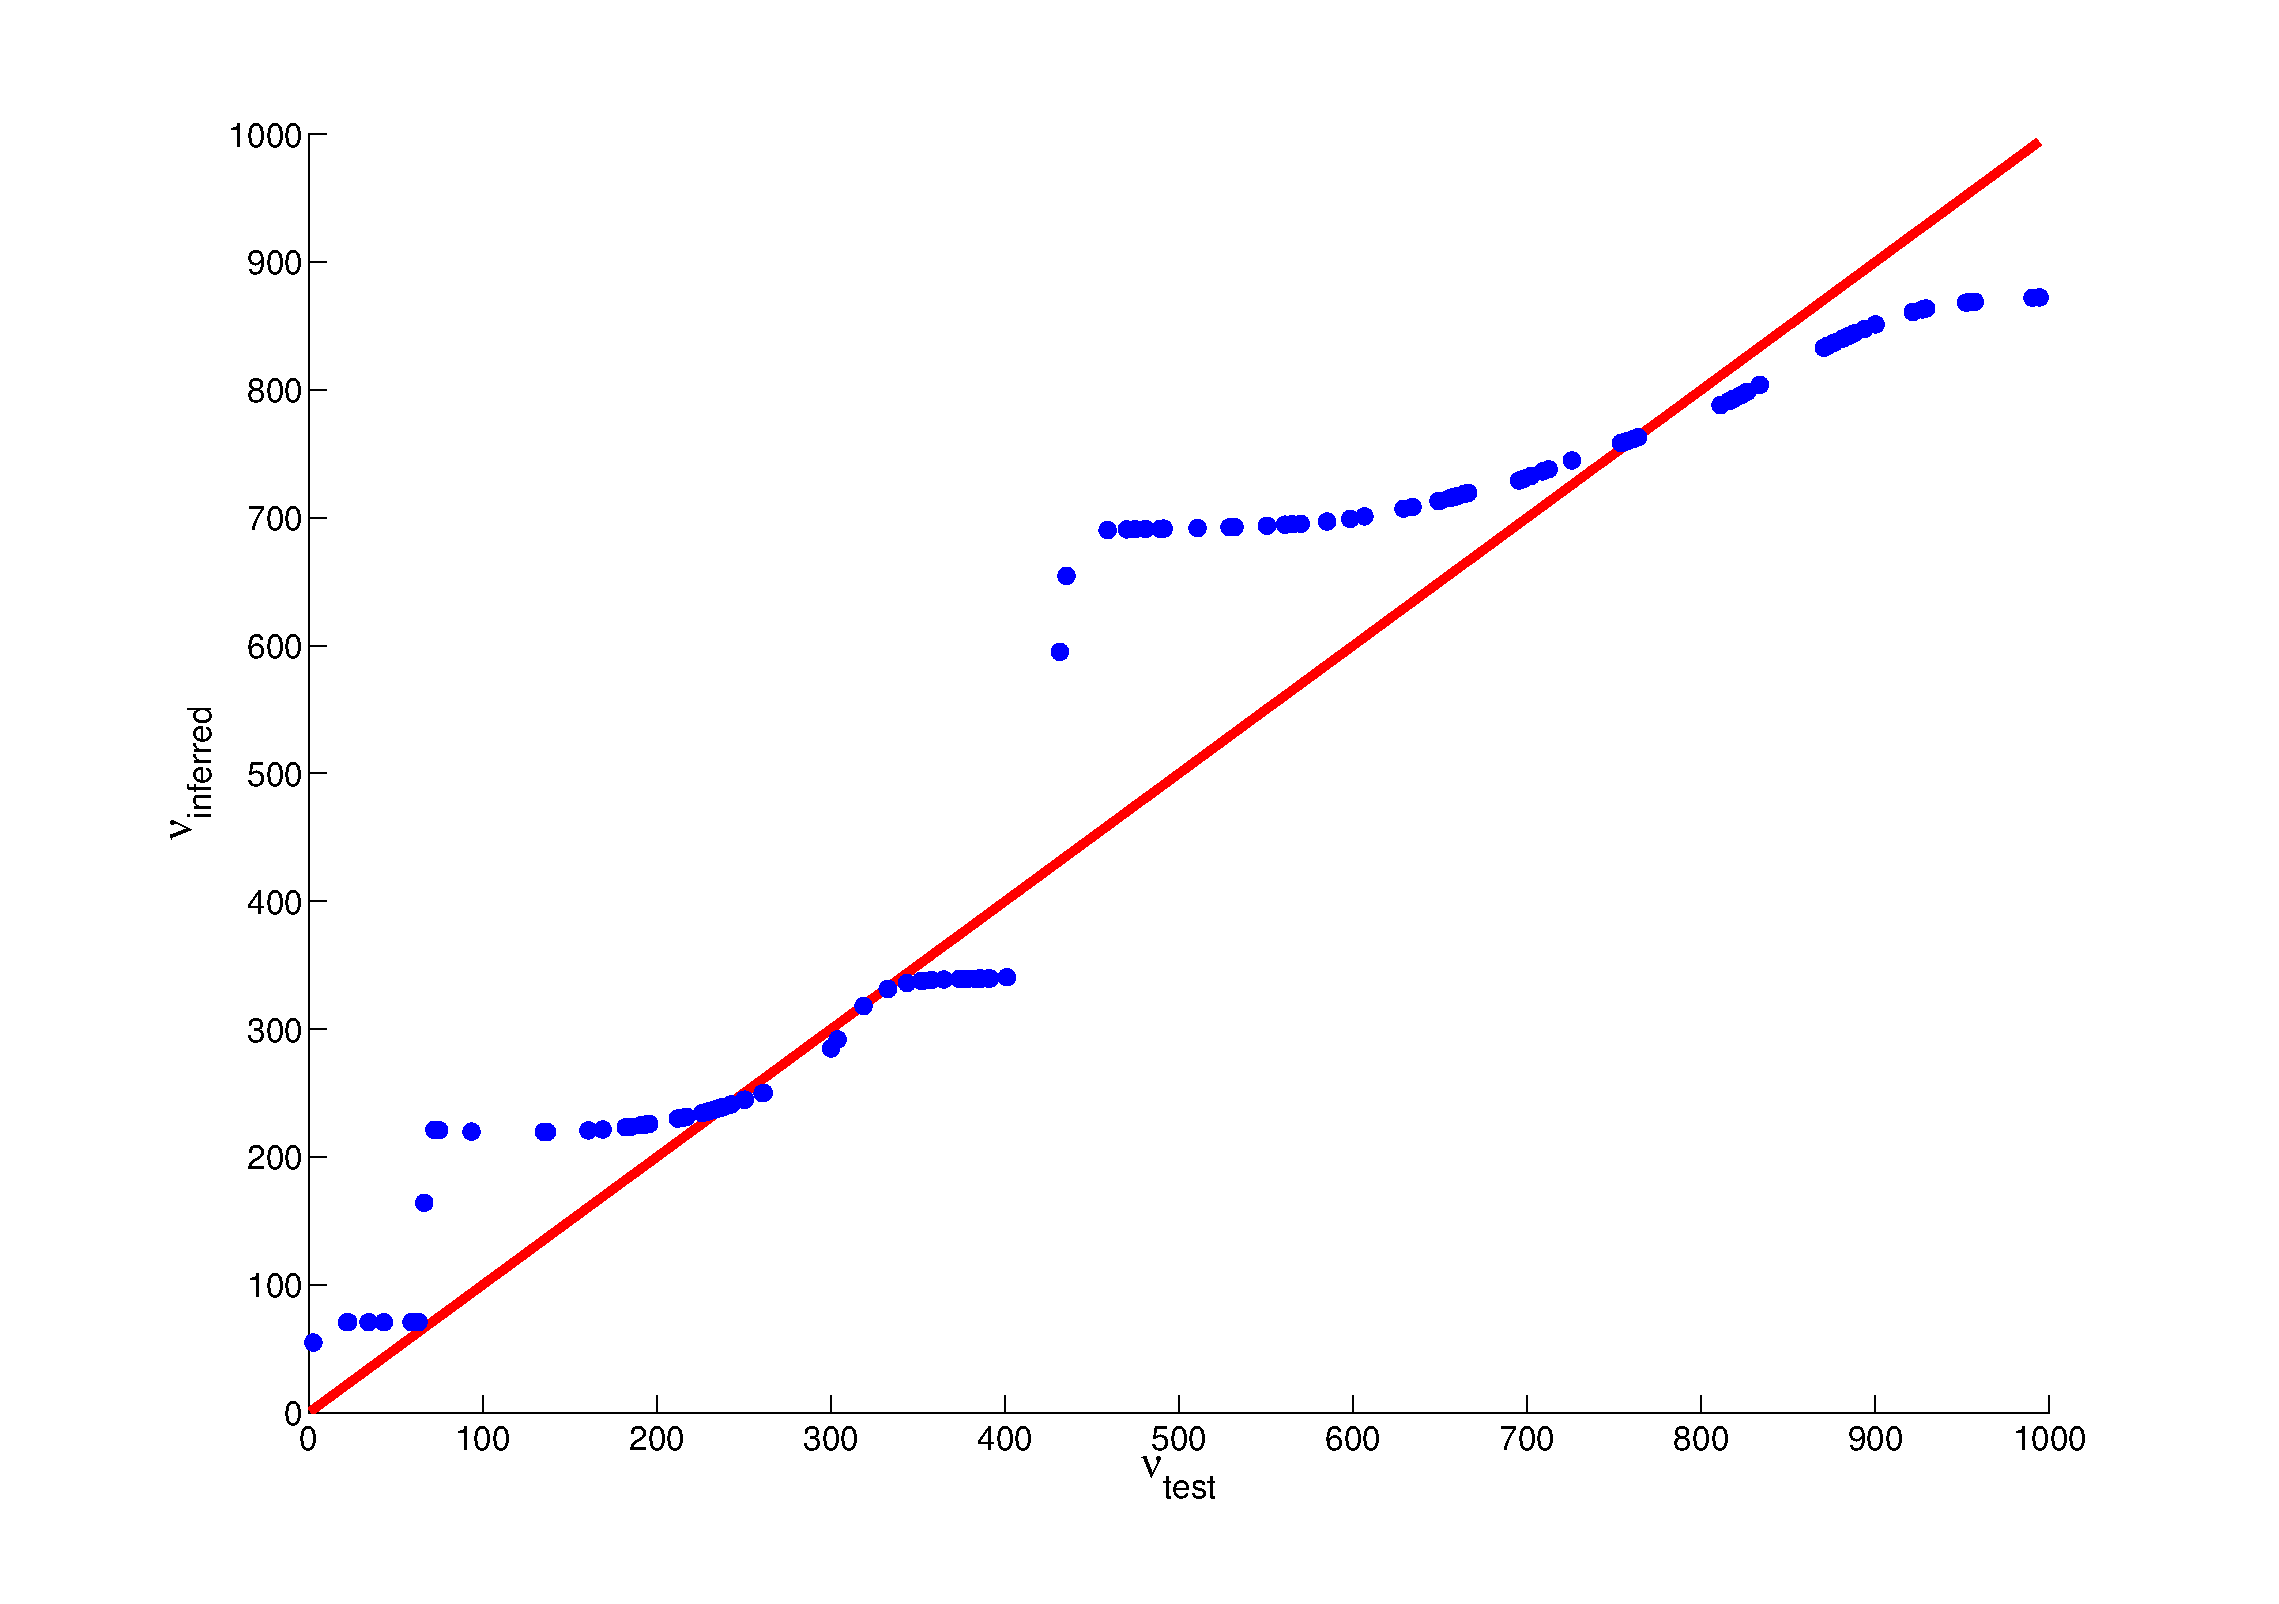
\includegraphics[width=\textwidth]{MN_small1.eps}
% tau4_M1.eps: 0x0 pixel, 300dpi, 0.00x0.00 cm, bb= -304   -42   height=100 mm
\begin{footnotesize}
 Figure 13, $M=15$, $N=10$
\end{footnotesize}
\end{center}

Figure 13 shows that the inferred input frequency is not well-matching with the actual test input frequency. There is not enough number of neurons to make the communication better.

\end{document}
